\documentclass{article}
\usepackage{amsfonts}
\usepackage{amsmath}
\usepackage{graphicx}
\usepackage{hyperref}
\usepackage{caption}
\usepackage{fancyhdr}
\usepackage{geometry}
	\geometry{height=24 cm}
	\geometry{left=2.5 cm}
	\geometry{right=2.5 cm}
	\geometry{top=2 cm}
	\geometry{headheight=1 cm}

\setcounter{secnumdepth}{2}


\title{\vspace{2cm}\textbf{Appunti di Architettura \\ degli Elaboratori}}
\author{\vspace{3mm}2 ottobre 2021}
\date{\vspace{3mm} \textbf{Rosso Carlo}}

\begin{document}

\begin{titlepage}
	\maketitle
	\thispagestyle{empty}
\end{titlepage}
\tableofcontents
\newpage

\section{Introduzione}

\newtheorem{definizione}{Definizione}[subsection]

All'inizio del corso studiamo le varie componenti di un computer da un punto di vista macroscopico e piano piano approfondiamo più nel dettaglio le varie parti che danno vita ad un PC.\\

Le componenti principali di un computer sono il \textbf{processore}, la memoria interna veloce, la \textbf{RAM}, che è volatile, una memoria esterna più lenta, ma molto più capiente, che conserva i dati anche quando il PC è spento; infine ci sono tutti i vari dispositivi di Input e Output (I/O). e.g. tastiera, mouse, display, casse...\\

In generale è bene fare un distinguo fin da subito: non è possibile avere una memoria capiente, veloce e di dimensioni ridotte poichè costerebbe molto. Le memorie capienti si basano su una tecnologia del tipo \textit{dynamic}, in quanto questa permette di compattare le celle di memoria. Il lato negativo di questa tecnologia è che si logora con il tempo: la lettura dei dati comporta la distruzione della memoria. D'altro canto le RAM sono del tipo \textit{static}, per cui sono meno compatte, ma più veloci. Questo spiega come mai le RAM di un computer fisso sono più economiche di quelle di un portatile: compattare le celle di memoria, senza rallentare o diminuire la capacità è costoso.

\subsection{Definizione di microprogrammazione}
	\label{microprogrammazione}
 La microprogrammazine è alla base di tutti i dispositivi che non sfruttano la tecnologia \textit{embedded system}, infatti questi calcolatori sono molto versatili e permettono di effettuare molte operazioni diverse. Un \textit{device} di questo tipo ha moltissimi circuiti che combinati permettono di svolgere operazioni diverse. Ad esempio l'Intel, un brand di processori, implementa un nuovo circuito ogni mese. Ad oggi negli ultimi processori ci sono circa 500 circuiti.\\

 Agli antipodi di questa tecnologia si trova l'\textit{embedded system} che sfrutta la programmazione camblata e quindi l'\textit{hardware}: non è possibile codificare un programma; questo viene "scritto" direttamente tramite i componenti e possono essere svolti solo calcoli predeterminati in un ordine preciso.\\

In un computer per ottenere le massime prestazioni possibili, bisogna sincronizzare tutte le funzioni così che mentre la CPU elabora, lo \textit{storage} legge o scrive e così via.
Perchè questo sia possibile nei computer si individua la componente di controllo. In realtà l'unità id controllo è divisa tra i vari componenti e li coordina.
Inoltre non dobbiamo dimenticare i bus, ovvero il mezzo di trasporto delle informazioni: i cavi elettrici.\\
Un aspetto interessante, nell'ambito dell'evoluzione dei PC, riguarda la compattezza dei vari strumenti che compongono un computer; per quanto possa sembrare banale, componenti più piccoli, implicano cavi elettrici più corti. Di fatto dimezzando la lunghezza di un cavo l'informazione arriva due volte più veloce, riducendo la lunghezza di un terzo, la velocità aumenta di 3 volte. Non solo, in questo modo i vari componenti necessitano anche di un minore quantitativo di energia per compiere il medesimo tragitto: la resistenza diminuisce. \\

Come accennavo precedentemente, la microprogrammazione \textit{de facto} rallenta il PC, per questo motivo sono caratterizzati dall'architettura \textbf{RISC}, per cui le istruzioni più utilizzate sono direttamente tradotte in hardware, in modo tale da rendere quei processi più rapidi.

\paragraph{L'architettura di un programma} per definizione è ciò che è esposto esternamente, proprio come la facciata di un edificio; insomma è il set di istruzioni.
\paragraph{L'organizzazione} si trova agli antipodi dell'architettura; per comprendere meglio adduco un esempio: nel 1970 uscì l'IBM, la versione pro, con tutti i componenti all'avanguardia, due anni dopo uscì una versione più lenta, ma assemblata nello stesso modo. Per intenderci i componenti non erano i migliori sul mercato per permettere a più aziende di acquistare il prodotto. In questo caso l'architettura era la stessa, mentre l'organizzazione era diversa.\\

Spieghiamo come mai bisogna comprare una macchina proporzionata, senza eccessi o difetti:
poichè la pipeline, \autoref{pipeline} avviene in modo simile ad una catena di montaggio, non ha senso assemblare un computer che per esempio ha un processore molto veloce, ma una RAM economica e quindi lenta. Riflettiamoci un momento: la CPU finirebbe di eseguire i calcoli prima che la RAM sia in grado di inviarle le informazioni successive e dunque il computer risulterebbe essere molto lento.
Tuttavia è vero anche il contrario: se il processore fosse troppo lento ad elaborare le informazioni, tutta la RAM immagazzinerebbe dati e si riempirebbe; un po' come quando si versa tanta acqua in un imbuto: se il buco dell'imbuto è troppo piccolo non ha senso aumentare le dimensioni della capacità dell'imbuto: non è quello il problema. Tuttavia a seconda delle funzioni che svolge un computer il bilanciamento delle componenti è diverso e dunque è bene informarsi sotto questo punto di vista prima di fare un acquisto.\\

Riassumento le funzionalità principali di un computer sono 4:
\begin{itemize}
	\item Elaborazione Dati, se ne occupa la CPU;
	\item Memorizzazione Dati, se ne occuma la memoria interna;
	\item Trasmissione Dati, se ne occupano gli I/O del caso;
	\item Controllo, si trova in ognuna delle funzionalità precedenti.
\end{itemize}

\paragraph{Definizione di Parola} \label{parola} 64 bit (oggi). Si tratta di una peculiatità che dipende dall'archittettura di un computer, un tempo una parola era molto più piccola. La parola coincide con la dimensione di un \textit{fixed point number}. Inoltre è comodo che la dimensione di una parola sia un multiplo di 8 bit in ASCII, il numero di bit necessario per identificare un carattere, in modo tale che possano essere memorizzate parole intere, indifferentemente dalla loro lunghezza.

E dunque \textbf{semiparola} = 32 bit

Il massimo valore esprimibile con i bit si calcola così:
\begin{equation} \label{valoremassimo}
	\max_{valore}= 2^n-1
\end{equation}
tale che $n=$ numero di bit, poichè ogni bit può contenere un 1 o uno 0 e si considera che siano tutti 1. \\
\noindent A ogni byte corrispondono 8 bit. In generale i byte sono utilizzati in riferimento alla memoria, perchè da un punto di vista econimico ha senso fare celle di memoria da 8 bit. Invece l'unità di misura delle informazioni è il bit (la velocità di connessione dei computer si misuta in $bit/s$, anche la velocità di trasferimento dati delle memorie esterne si misura in $bit/s$)
\newline

\begin{table}[h]
	\centering
	\begin{tabular}{|c|c|c|c|c|}
		\hline
		  &  &  &  &  \\
		Kilobyte & Megabyte & Gigabyte & Terabyte & Petabyte \\
		  &  &  &  &  \\
		\hline
		  &  &  &  &  \\
		$2^{10}$ bytes & $2^{20}$ bytes & $2^{30}$ bytes & $2^{40}$ bytes & $2^{50}$ bytes \\
		  &  &  &  &  \\
		\hline
	\end{tabular}
	\caption{Tabella di conversione dei byte}
\end{table}

\subsection{Definizione di Cablato}
	I programmi cablati sono fatti sull'hardware, vedi \autoref{microprogrammazione}, in particolare si tratta degli \textit{embedded system}.

In questi casi non è possibile cambiare programma, però possiamo inserire dati diversi ed elaborare la medesima operazione. Si tratta di programmi molto veloci, ma non flessibili.

\subsection{Definizione di Programmazione Software}

La programmazione software, consiste in un hardware generico accompagnato da alcuni dati salvati in memoria, che si dividono nei dati di input dell'operazione e nella lista di istruzioni da eseguire con quegli input.



In questo caso il processore sarà diverso dal sistema cablato: sarà dotato di una memoria propria che gli consente di avere i dato di input a portata di mano e il percorso che queste informazioni devono eseguire, inoltre deve avere la possibilità di memorizzare l'output per poi rimandarlo alla RAM. Bisogna ricordare che sia i dati di input che le istruzioni sono codificate in bit e duque devono essere decodificate e poi mandate all'ALU.

\section{La CPU}
Più nel dettaglio la CPU è formata da:
\begin{itemize}
	\item ALU (\textit{arithmeric and logic unit}), c'è un'ALU per core;
	\item IR (\textit{instruction register}), ricorda l'istruzione ora in esecuzione nell'ALU;
	\item PC (\textit{program counter}) \label{programcounter}, ricorda l'indirizzo dell'istruzione in esecuzione e conta i programmi eseguiti;
	\item MAR \textit{memory address register}, qui sono è salvato l'indirizzo dell'ultimo dato richiesto dalla CPU, il MAR è connesso con la \textit{cache} e quindi con i componenti al di fuori della CPU (canale di uscita);
	\item MBR (\textit{memory buffer register}), riceve tutte le informazioni che provengono dalla \textit{cache} o dagli altri componenti (canale di entrata);
	\item I/O AR (\textit{i/o address register}), come il MAR, ma solo per i dispositivi di input e output;
	\item I/O BR (\textit{i/o buffer register}), come l'MBR, ma solo per i dispositivi di input e output.
\end{itemize}

Nell'architettura I/O mapping l'\textit{I/O adress register} e l'\textit{I/O buffer register} non sono necessari, infatti gli indirizzi per riferisi alle celle di memoria della RAM o dei dispositivi esterni sono accorpati assieme. ++(Il motivo per cui siamo passati da una stuttura a $16 bit \rightarrow 32 bit \rightarrow 64 bit$ è che le memorie si sono evolute talmente tanto che in 32 bit non eravamo più in grado di indicare tutti gli address disponibili.)

\subsection{Processi della CPU}
\label{cicloistruzione}

\begin{figure}[h]
	\centering
	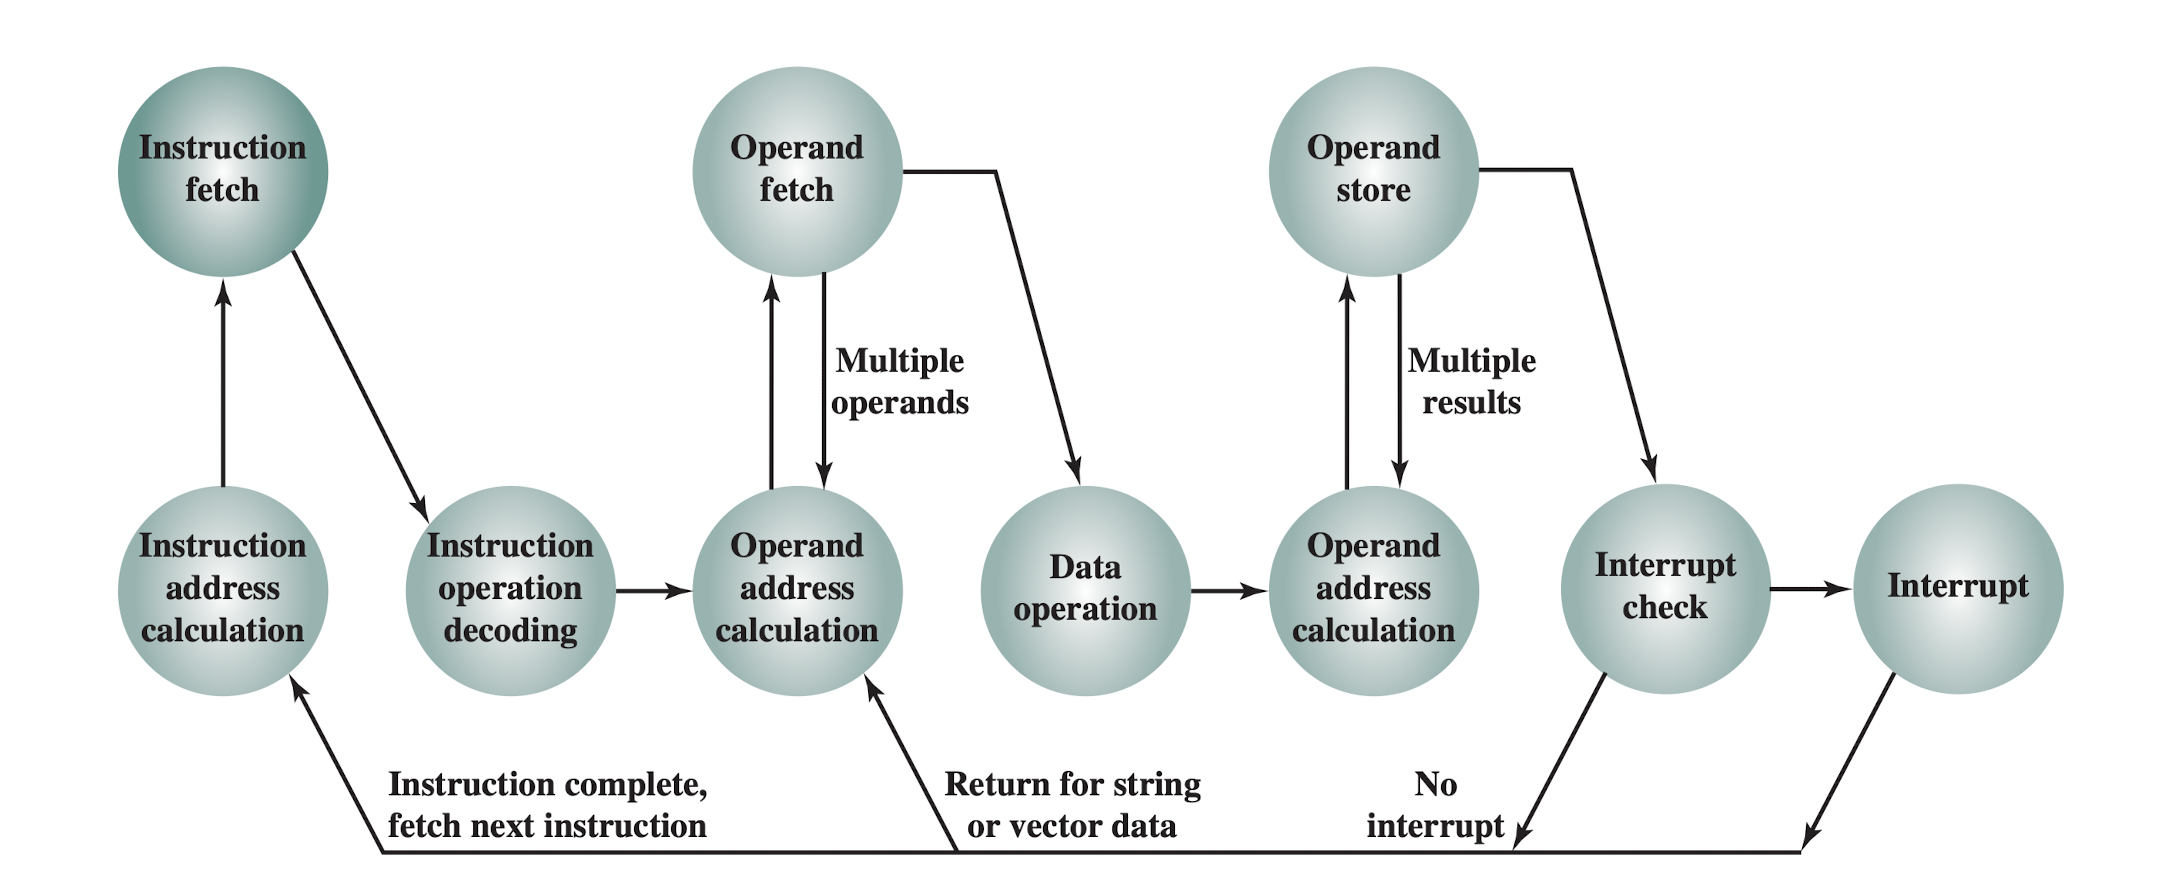
\includegraphics[scale=0.3]{immagini/cicloistruzioni}
	\caption{Ciclo di esecuzione di un'istruzione}
\end{figure}

Ora descriviamo in breve quali sono le fasi di esecuzione di un'istruzione.
\begin{enumerate}
	\item fetch dell'istruzione: la CPU pone l'indirizzo dell'istruzione da eseguire nel MAR(memory address register) e riceve l'istruzione dalla RAM;

	\item instruction operation decoding: l'istruzione è prelevata dall'MBR(memory buffer register) ed è posta nell'IR(instruction register), qui è decodificata;

	\item operand address calculation: la CPU calcola gli indirizzi in cui sono contenuti i dati che sono elaborati;

	\item operand fetch: l'indirizzo precedentemente calcolato è posto nel MAR in modo tale da ricevere gli operandi dalla RAM nell'MBR;

	\item data operation: l'ALU effettua l'operazione logico aritmetica, se richiesta;

	\item operand address calculation: è calcolato l'indirizzo in cui salvare il risultato;

	\item operand store: il risultato viene posto nella cella di memoria indicato;

	\item interrupt check: la CPU controlla se l'unità di controllo ha ricevuto deggli interrupt;

	\item interrupt: se la CU (control unit) ha ricevuto un interrupt allora sono recuperate le informazioni necessarie per risolvere il problema;

	\item instruction address calculation: è calcolato l'indirizzo della prossima istruzione, in modo tale che il ciclo possa ricominciare.
\end{enumerate}


\subsection{La priorità} \label{priorita}
La CPU una volta finito un programma ha il compito di mandarlo al \textbf{modulo di controllo output} che si occupa di mostrare il risultato, che sia sonoro, o una stringa, oppure un video. Per fare questo, essa stessa deve compiere alcuni processi che devono essere sincronizzati con il sistema di output che è generalmente molto lento rispetto al processore. Per questo motivo mentre l'output si sincronizza con la CPU, quest'ultima cotinua a processare dati di altri programmi ottimizzando le tempistiche; appena il dispositivo è pronto la CPU interrompe la serie di funzioni che sta svolgendo per elaborare i dati di output. Per effettuare questa operazione all'interno della CPU sono contenute delle memorie in grado di ricordare momentaneamente le informazioni del programmma che è stato messo in pausa, in modo tale che il processore sia sempre in grado di tornare a svolgere un altro programma nei "momenti morti".

\begin{figure}[ht]
	\centering
	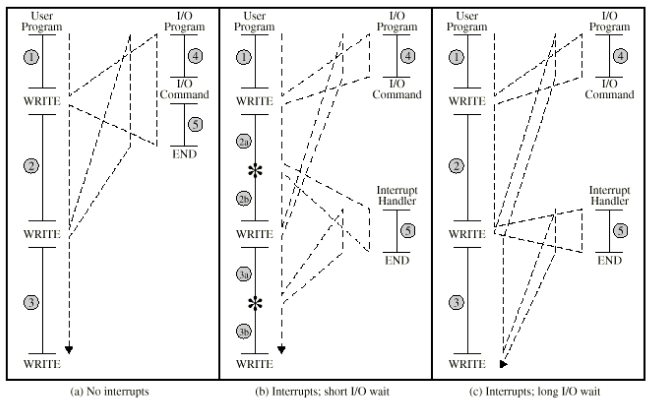
\includegraphics[scale=0.3]{immagini/ottimizzazione_cpu}
	\caption{lo stesso programma viene ottimizzato in modo diverso}
\end{figure}

Il medesimo processo avviene quando un programma con una priorità maggiore rispetto a quello in esecuzione deve essere completato. Tutto ciò previene perdite di dati o rallentamenti di sistema. Il segnale di interruzione arriva dalla memoria periferica oppure dal controllo I/O (il segnale di interrupt viene mandato alla CPU, quindi è chiaro che sia una componente esterna a mandarlo).

\subsection{Il BUS}
Il bus, a livello hardware, è composto da tutti i cavi elettrici che permettono le comunicazioni tra i componenti di un elaboratore. Il bus è in grado di condividere multipli di parola per volta; la dimensione di una parola dipende dall'architettura del calcolatore. Inizialmente c'era solo il bus di sistema che mette in comunicazione i moduli di I/O con la CPU e la memoria principale; il bus è costruito in modo tale da permettere ad ogni componente di comunicare contemporaneamente a tutti gli altri. In altre parole, i dati sono condivisi solo da un componente per volta: è come una chiamata, se ci sono tante persone e tutte parlano non si capisce nulla; bisogna stabilire delle regole e permettere solo ad un individuo per volta di comunicare. Per questo motivo è implementato l'arbitro del bus nei PC ed esso gestisce le comunicazioni tra i componenti. Per organizzare le comunicazioni il bus è diviso in tre livelli ben distinti:
\begin{itemize}
	\item bus dati: su questo bus si condividono i dati tra i vari componenti;

	\item bus indirizzi: su questo bus si condividono gli indirizzi di cui la CPU ha bisogno;

	\item bus segnali di controllo: in questo livello si comunica con l'arbitro del bus per prendere il controllo del bus (bus grant e bus request); su questo bus la CPU indica se ha bisogno di leggere o scrivere dei dati (read e write); oppure la CPU e il modulo di I/O si sinconizzano; su questo livello sono mandati gli interrupt.
\end{itemize}

Il bus si è evoluto parecchio nel tempo, per esempio, quando fu introdotta la gerarchia di memoria, fu inventato il \textbf{local bus} che permette la comunicazione tra \textit{cache} e \textit{core}; oppure con l'avvento delle connessioni LAN, alcuni dispositivi di I/O sono diventati molto più veloci di altri, come la stampante o il fax. Per questo motivo sono stati introdotti: il \textit{bus ad alta velocità}, attraverso cui passano i dati tra i moduli di I/O più veloci e la \textit{cache} ed il \textbf{bus di espansione}, in cui sono accumulati tutti i dispositivi più lenti. A causa del numero di dispositivi e della loro lentezza, si forma un collo di bottiglia sul dispositivo che regola le informazioni tra bus di espansione e bus ad alta velocità (torneremo su questo discorso alla \autoref{i/o}).

\begin{figure}[h]
	\centering
	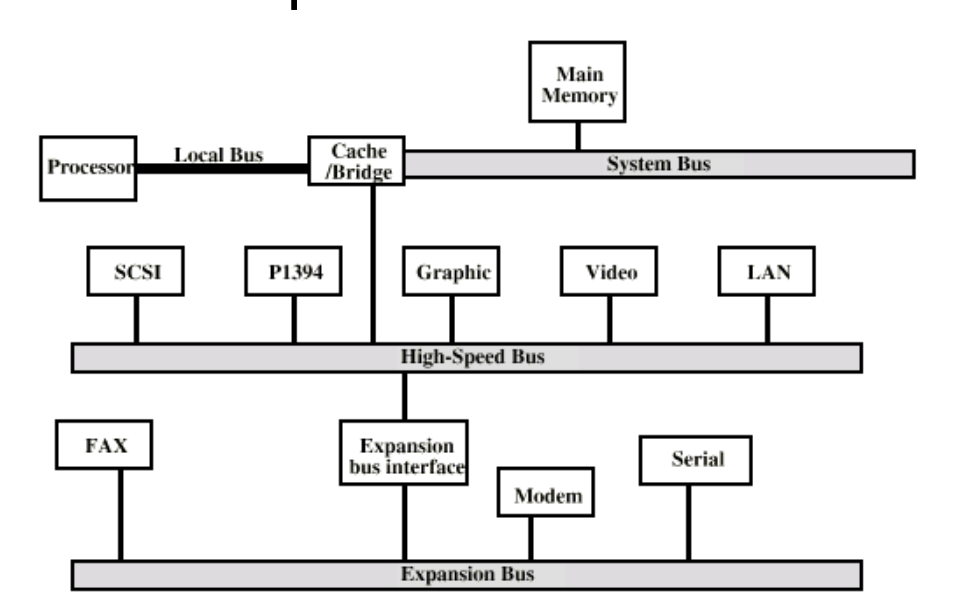
\includegraphics[scale=0.3]{immagini/bus_immagine_esemplificativa}
	\caption{I bus nei computer moderni}
\end{figure}

Un altro argomento molto interessante legato ai bus riguarda i processori multi\textit{core}: ogni \textit{core} è un chip di elaborazione dati, molto simile ad una CPU.
In questo caso, i multi\textit{core} più all'avanguardia dispongono di bus per comunicare informazioni a singoli \textit{core}, si tratta di bus punto a punto. Bisogna aggiungere che ogni \textit{core} è dotato dei propri registri, cioè della propria \textit{cache}, e ciascuna è in grado di comunicare con le altre. Perchè questo sia possibile, è stato introdotto un \textbf{sistema a crediti} che segnala alla \textit{cache} con la quale si comunica quanto spazio resta nel \textit{buffer}. Non solo per ogni collegamento con altri \textit{core}, ogni \textit{core} ha una \textit{cache}, questo vuol dire che ogni CPU ha diverse \textit{cache}. \\
Quando una \textit{cache} di un \textit{core} si riempie, ma non sono arrivate tutte le informazioni richieste, i dati cambiano percorso arrivando così sullo stesso \textit{core}, ma in un altra cache. Per fare questo è stato pensato il \textit{router}, il sistema di instradamento dei dati, che tiene conto dei crediti e indirizza le informazioni attraverso i bus disponibili, così da non sovracaricare i registri dei \textit{core}.\\
Un altro punto importante è il livello \textit{link}: consiste in un livello di controllo del codice tramite il software a bassissimo livello; agisce in questo modo: i \textit{core} si mandano 80 bit di dati per volta, 8 sono di controllo dei restanti 72 e permettono di capire se ci sia un errore o se vada tutto bene. Se è stato commesso qualche sbagli il pacchetto è mandato di nuovo e così per tutti i pacchetti successivi. I crediti sono possibili proprio grazie al livello \textit{link}.\\
In aggiunta in ogni buffer c'è un \textit{firmware} che consiste in dati già pronti per essere inviati per segnalare errori e quant'altro. Poichè il \textit{firmware} è composto da dati salvati nei registri è aggiornabile e quindi è molto flessibile, se si trattasse di un componente hardware andrebbe sostituito il pezzo.

\section{La memoria}

La memoria ha diverse caratteristiche:
\begin{itemize}
	\item locazione;
	\item capacità;
	\item metodo di accesso, che si divide in:

	\begin{itemize}
		\item sequenziale(nastro, lenta ma capiente, le liste in python);
		\item diretto(gruppi e poi sequenziale);
		\item casuale(come i set() in python);
		\item associativo(come dict());
	\end{itemize}

	\item prestazioni;
	\item modello fisico:

	\begin{itemize}
		\item ottico;
		\item magnetico;
		\item semiconduttore;
		\item magnetico-ottico;
	\end{itemize}

	\item volatile, o non; rw o non;
	\item organizzazione, com'è divisa.
\end{itemize}

In generale l'ampiezza e le prestazioni di una memoria sono inversamente proporzionali a causa del costo proibitivo. \\
Fatto interessante: se le CPU sono mille volte più veloci rispetto a quelle che erano usate negli anni `80, la velocità dei registri non è aumentata nemmeno di 10 volte. Infatti fino a poco tempo fa non erano necessarie memorie più veloci, invece si è sempre aggirato il problema grazie gerarchia di memoria.
Per questo motivo oggi nei computer si usano tante memorie diverse in base all'utilizzo. Per esempio i processori moderni sono dotati di 3 livelli di registri; le informazioni di cui ha bisogno l'ALU sono contenute nel più piccolo che è collegato ad uno appena più grande, ma più lento, fino a che non si arriva al registo collegato direttamente alla cache. Tra il l'ALU e il registro più piccolo sono trasferiti pochi dati per volta, ma molto velocemente, tra l'ultima \textit{cache} e lo \textit{storage} sono trasferiti blocchi di informazione molto grande. Questo perchè la memoria interna è molto lenta e a cause del modo in cui le informazioni sono salvate in essa: tendenzialmente le prossime informazioni che serviranno alla CPU sono contenute vicina alle precedenti.

\subsection{L'accesso in memoria}

I computer odierni implementano più memorie che collaborano per ottenere prestazioni maggiori ad un prezzo inferiore. A ogni riga in \textit{cache} corrisponde un blocco di dati, e quindi una potenza di 2 di parole. Per trovare i dati all'interno della cache possono essere utilizzate tre tecniche:
\begin{enumerate}
	\item \label{Directmapping} \textbf{Associazione Diretta:} in questo caso l'indirizzo di memoria è diviso in tre parti, il tag, la line e la word. La line serve per conoscere in quale riga della cache cercare la parola in questione; il tag permette di capire se nella riga in questione c'è il blocco che cerchiamo; ed infine la word ci indica quale parola stiamo cercando all'interno del blocco. In pratica:
	\begin{itemize}
		\item $j$: indirizzo di memoria;

		\item $m$: numero di righe della cache e numero di blocchi che può contenere nello stesso momento;

		\item $i$: riga in cui si trova il blocco;

		\item $w$: $2^w$ n. parole contenute in un blocco, $w$ serve per indentificare la parola nel blocco;

		\item $j//m$: tag, serve per individuare il blocco.
	\end{itemize}

	\item \label{Associativemapping} \textbf{Associazione Completa:} in questo caso il nuovo blocco è inserito nella prima riga disponibile. Questo metodo permette di matenere gli ultimi blocchi caricati nella \textit{cache} anche se con una divisione di modulo $m$ dovrebbero essere riscritti. A parte questo vantaggio, non è possibile conoscere la riga a priori e dunque è necessario conotrollare ogni tag per vedere se la \textit{cache} ha il blocco richiesto. Ricapitolando:
	\begin{itemize}
		\item $j$: indirizzo di memoria;

		\item $w$: come prima;

		\item $j-w$: tag, serve per identificare il blocco.

	\end{itemize}

	\item \label{SetAssociativeMapping} \textbf{Set-Associative mapping:}
	La memoria è divisa in set ed in ogni set ci sono più righe. Per decidere in quale set memorizzare un blocco si esegue una divisione in modulo $m/k$, dove $m$ è il numero totale di set all'interno della \textit{cache}. Dunque un blocco è salvato all'interno di un set con l'\textit{associative mapping method}. In questo caso è veloce ricercare la riga in cui è presente il blocco che cerchiamo poichè si cercherà tra i tag in un certo set. In questo modo sono tenuti gli ultimi blocchi che corrispondono allo stesso set e la ricerca dei tag è veloce. Ricapitolando:
	\begin{itemize}
		\item $j$: indirizzo di memoria;

		\item $m$: numero di righe della cache, numero di blocchi che può contenere nello stesso momento;

		\item $k$: numero righe per set;

		\item $i$: set;

		\item $w$: $2^w$ n. parole contenute in un blocco, $w$ serve per indentificare la parola nel blocco;

		\item $j//(m/k)$: tag, serve per individuare il blocco.
	\end{itemize}

Per risolvere gli esercizi che riguardano il \ref{SetAssociativeMapping} è utile ricorrere alle seguenti formule:
\begin{enumerate}
  \item Blocco: si calcola dividendo la dimensione del blocco per la dimensione di una parola;

  \item word: per conoscere quanti bit sono necessari per individuare una parola è sufficiente risolvere il $\log_2(x)$ dove $x$ è il numero di parole in ciascun blocco;

  \item Linee: per conoscere quante linee sono disponibili in \textit{cache} si divide la dimensione della \textit{cache} per la dimensione di un blocco. Questo valore coincide con il numero di blocchi che la \textit{cache} è in grado di memorizzare nel medesimo momento;

  \item n. set: per conoscere quanti set ci sono nella \textit{cache} bisogna dividere la variabile Linee, precedentemente vista, per il numero di vie che caratterizza l'architettura;

  \item set: per calcolare il numero di bit necessari per individuare un set si calcola il $\log_2(x)$, dove $x$ è il numero di set precedentemente calcolato;

  \item address: per conoscere la lunghezza di un indirizzo è sufficiente conoscere il $\log_2(x)$, dove $x$ è la grandezza della memoria;

  \item tag: per calcolare il tag bisogna sottrarre all'address la word e il set.
\end{enumerate}

\end{enumerate}

\paragraph{Gerarchie di memoria.} A questo riguardo sorge spontanea una domanda: dal momento che la \textit{cache} non è ampia quanto la RAM, in quale modo si selezionano i blocchi che restano nella \textit{cache} e quelli che vengono riscritti? (Ovviamente il quesito si pone solo per \ref{Associativemapping} e \ref{SetAssociativeMapping}). Ci sono quattro metodi principali attraverso cui scegliere quali blocchi tenere e quali eliminare:
\begin{enumerate}
	\item \textbf{Casuale}, per occupazione omogenea dello spazio, il più semplice;

	\item \label{fifo} First-in-First-Out (\textbf{FIFO});

	\item Least Frequently Used (\textbf{LFU});

	\item Least Recently Used (\textbf{LRU}).

\end{enumerate}

\subsection{DRAM}

Come anticipato prima, esistono varie tipologie di memoria, in particolare ogni PC è dotato di alcune memorie volatili molto veloci; La più capace si chiama RAM e ci siamo riferiti ad essa chiamandola memoria principale. RAM è l'acronimo di \textit{Random Access Memory}, proprio perchè funziona ad accesso casuale. A causa del prezzo elevato di alcune RAM i computer oderni tendono ad incorporare varie tipologie per ottenere buone prestazioni ad un costo minore. In particolare oggi le memorie si dividono in DRAM (\textit{Dynamic $\dots$}) e in SRAM (\textit{Static $\dots$}).\\

La DRAM memorizza un bit caricando le piastre di un condensatore; quando si ha la necessità di conoscere l'informazione si apre il circuito ed uno strumento misura il flusso di corrente. Se c'è poca corrente allora il segnale sarà 0, altrimenti sarà 1. Il condensatore tende a scaricarsi col tempo, per questo motivo è necessario il \textit{refresh} e quindi le DRAM sono lente. Le DRAM in genere vanno a formare la memoria principale, la RAM.

\subsection{SRAM}\label{sram}

La SRAM è una memoria che ha un funzionamento più complesso e ha bisogno di più spazio, ma al contrario della DRAM può essere letta in qualunque momento: non ha bisogno del \textit{refresh}. Poichè il circuito di una SRAM è più complesso è anche più caro. Tendenzialmente le SRAM svolgono il ruolo di \textit{cache} (memorie molto piccole e molto veloci).

\section{ROM}

Oltre alle memorie volatili ci sono anche sistemi di memorizzazione permanenti: è il caso delle ROM (\textit{Read Only Memory}, per cui in realtà si traduce come, memorie principalmente in lettura). Le ROM sono state sotituite dalle PROM (\textit{Progmammable $\dots$}), che possono essere scritte in un secondo momento. Dopo le PROM è venuto il momento delle EPROM (\textit{Erasable $\dots$}), che permettono più flessibilità: possono essere riscritte. Ed infine sono state introdotte le \textbf{EEPROM} (\textit{Electrically Erasable Programmable Read-Only Memory}). In questo caso è possibile formattare anche singoli byte, e dunque la memoria diventa molto flessibile, ma lenta.\\

Un'altra tecnologia interessante riguarda le memeorie \textit{\textbf{flash}}: hanno una capacità paragonabile a quella delle EPROM, ma si può decidere quali blocchi tenere e quali blocchi cancellare in pochi secondi.

\section{Correzione di un solo errore, Hamming Code}
\label{hammingcode}

Il metodo Hamming Code rende possibile correggere un singolo errore in un codice binario e permette di individuare due eventuali sbagli. Se abbiamo un codice formato da $m$ bit, per prima cosa abbiamo bisogno di conoscere quanti bit di controllo sono necessari per verificare la correttezza del codice; in aggiunta non dobbiamo dare per scontato che solo il codice che abbiamo sia scorretto, anche il codice di controllo potrebbe contenere un errore. Diciamo che il codice di controllo sia lungo $m$ bit, allora dobbiamo controllare $m + k$ bit. Ogni bit di controllo è in grado di correggere 2 bit, però combinati sono in grado di controllare $2^k-1$ bit e dunque per sapere quanti bit di controllo sono necessari bisogna risolvere la seguente disequazione:
\begin{equation}
	2^k>m+k
\end{equation}
Dove $m$ corrisponde al numero di bit di informazioni utili e quindi si tratta di una potenza di 2.\\

In breve l'\textit{hamming code} funzina nel seguente modo:
\begin{enumerate}
	\item Ad un codice binario di lunghezza m bit è associato un codice di correzione di errore singolo di lunghezza k. Si ricordi che le informazioni mandate devono sempre essere potenze di 2, per questo motivo i codici mandati non sono mai potenze di 2: ai bit di dati bisogna sommare i bit di correzione di errore. Mentre l'informazione in memoria è salvata come potenza di 2, il codice binario mandato dalla memoria avrà ad esso aggiunto un codice di correzione di lunghezza k che è calcolato dalla memoria;

  \item Il codice di correzione è inserito in mezzo ai dati nelle posizioni che sono potenze di 2. Per esempio un codice di errore avrà i propri bit nel primo, secondo, quarto, ottavo, sedicesimo, ... bit;

	\item Il valore del bit di correzione è sceltro attraverso l'operazione xor, tra i valori delle posizioni che controlla. Per esempio se controlla i valori: 1,0,0,0,1,1,0,0,1 il suo valore sarà 0. In questo modo uno xor tra il codice di correzione e i valori che controlla sarà sempre 0. Se così non dovesse essere vuol dire che il codice di correzione oppure una delle caselle che controlla è errata;

	\item Per comprendere quali caselle controlla quale bit di correzione è comodo scrivere le varie posizioni in codice binario. Poniamo che ci siano 12 caselle di memoria e le informazioni da mandare siano contenute in un byte allora la posizine della prima casella si scriverà $0001$, la seconda $0010$, la terza $0011$, ...
	Si nota che i multipli di 2 hanno sempre e solo un 1 all'interno della propria posizione in binario;

	\item Il primo bit di correzione controlla tutte le posizioni che hanno un 1 alla fine. Il secondo bit di correzione controlla tutte le posizioni che hanno un 1 in seconda posizione, ...;

	\item Se l'errore si verifica all'iterno del codice di dati allora più di un codice di errore riferà che è avvenuto uno sbaglio. Se solo un bit è sbagliato allora l'errore consiste proprio nel valore del bit di correzione.

\end{enumerate}

Per esempio avendo il byte [10110100], lo riscriviamo in una tabella indicando la posizione dei bit, vedi \autoref{BEsercizio}.

\begin{table}[h]
	\centering
	\begin{tabular}{|c|c|c|c|c|c|c|c|c|c|c|c|}

		\hline
		&  &  &  &  &  &  &  &  &  &  & \\
	  12 & 11 & 10 & 9 & 8 & 7 & 6 & 5 & 4 & 3 & 2 & 1  \\

		1100 & 1011 & 1010 & 1001 & 1000 & 0111 & 0110 & 0101 & 0100 & 0011 & 0010 & 0001 \\
	  &  &  &  &  &  &  &  &  &  &  &  \\
		\hline
		&  &  &  &  &  &  &  &  &  &  &  \\

    1 & 0 & 1 & 1 & - & 0 & 1 & 0 & - & 0 & - & -\\

		&  &  &  &  &  &  &  &  &  &  &  \\
		\hline

	\end{tabular}
	\caption{Valore dei bit dati e relativa posizione nel codice che è mandato.}
	\label{BEsercizio}
\end{table}

Ora dobbiamo calcolare i bit che mancano al codice. Innanziutto calcoliamo che $k=4$ sia corretto e non siano necessati più o meno bit per controllare il byte che stiamo mandando:

\begin{equation*}
		2^4-1>8+4 \iff 15>12
\end{equation*}

Si nota che inviando un byte sono necessari proprio 4 bit di correzione.\\
Ora calcoliamo il primo bit:

\begin{gather*}
	value(0001) = value(0011) \oplus value(0101) \oplus value(0111) \oplus value(1001) \oplus value(1011) \\
	1 = 0 \oplus 0 \oplus 0 \oplus 1 \oplus 0
\end{gather*}
Il secondo bit invece corrispode a:
\begin{gather*}
	value(0010)= value(0011) \oplus value(0110) \oplus value(0111) \oplus value(1010) \oplus value(1011) \\
	0 = 0 \oplus 1 \oplus 0 \oplus 1 \oplus 0
\end{gather*}

 E così via. In questo modo il bit 4 ha valore 0 e controlla le caselle 5,6,7 e 12; mentre il bit 8 ha valore 1 e controlla le caselle 9,10,11 e 12.

 Quindi riscriviamo la tabella con i valori appena calcolati:

 \begin{table}[h]
 	\centering
	\begin{tabular}{|c|c|c|c|c|c|c|c|c|c|c|c|}

		\hline
		&  &  &  &  &  &  &  &  &  &  & \\
		12 & 11 & 10 & 9 & 8 & 7 & 6 & 5 & 4 & 3 & 2 & 1  \\

		1100 & 1011 & 1010 & 1001 & 1000 & 0111 & 0110 & 0101 & 0100 & 0011 & 0010 & 0001 \\
		 &  &  &  &  &  &  &  &  &  &  &  \\
		\hline
		&  &  &  &  &  &  &  &  &  &  &  \\

	   1 & 0 & 1 & 1 & 1 & 0 & 1 & 0 & 0 & 0 & 0 & 1\\

		&  &  &  &  &  &  &  &  &  &  &  \\
		\hline

	\end{tabular}
 	\caption{Byte di dati di esempio e relativo codice di errore.}
 \end{table}

\section{Le memorie esterne}

\subsection{I dischi magnatici}

I dischi magnetici sono una tecnologia che ha cominciato a diffondersi a partire dagli anni `80. Esistono numerose tipologie di dischi magnetici, per cui in introduzione cominciamo a descrivere le caratteristiche in comune a tutti quanti.\\
\indent I dischi magnetici sono composti da un substrato non magnetico come l'alluminio o più recentemente il vetro, più uniforme, resistente e liscio; possono immagazzinare un gran numero di informazioni e sono in grado di modificare i contenuti al proprio interno una volta scritti.
Le operazioni di lettura e scrittura avvengono grazie ad una testina attraversata da corrente, mentre il disco gira a gran velocità.\\
\indent La memoria all'interno dei dischi è divisa in cerchi concentrici che si chiamano tracce. Ogni traccia è poi divisa in settori. In genere il numero di tracce e di settori è una potenza di 2. Tra le tracce e i settori ci sono degli spazi per poter leggere le informazioni evitando errori.

\begin{figure}[h]
	\centering
	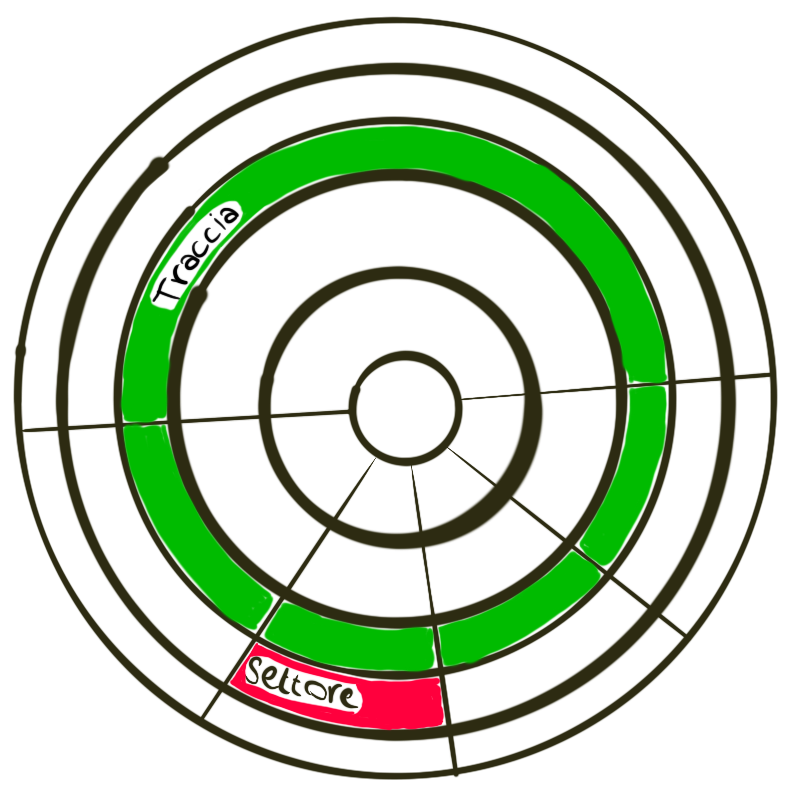
\includegraphics[scale=0.3]{immagini/cdrom}
	\caption{l'organizzazione della memoria dei cd.}
\end{figure}

\indent Alcuni dischi sono dotati di una velocità angolare costante: CAV, \textit{constant angular velocity}, tuttavia per questo motivo la densità di informazione all'interno del disco è disomogenea: agli estremi la velocià lineare è maggiore e dunque le informazioni salvate sono di meno a parità di volume. Per questo motivo è stata introdotta la tecnologia MZR: \textit{multiple zone recording}. Con la MZR si calcola la velocità in base alla posizione della testina in modo tale da rendere le informazioni più dense. In questo caso la memoria è divisa in diverse zone che contengono la medesima quantità di dati.\\
\indent Come anticipavo precedentemente, ci sono molte proprietà che può avere un disco:
\begin{enumerate}
	\item testina mobile/ fissa. Nel caso le testine sinao fisse sono disposte in modo tale da leggere tracce diverse e coprire l'intero disco;

	\item disco rimovibile o non rimovibile;

	\item double sided/ single-sided;

	\item multiple platters. In questo caso la memoria è divisa anche in cilindri, per cui la stessa traccia in dischi diversi forma un cilindro.
\end{enumerate}

 Innanzitutto per spiegare il funzionamento di dischi diversi bisogna comprendere che più la testina è piccola e più deve essere vicina al disco: i campi magnetici sono inversamente proporzionali al quadrato della distanza tra due punti; d'altro canto più la testina è piccola e più è precisa e allora lo stesso disco diventa più capace.
 Quindi riassumendo ci sono i primi dischi, che hanno velocità costante, ma densità di informazione diversa. Quindi sono stati inventati i dischi n.2: MZR. \\
 \indent Infine sono stati introdotti i Manchester Disk. Quando la memoria esterna è scollegata dalla corrente la testina è a contatto con il disco, tuttavia nel momento in cui il disco comincia a girare grazie all'aereodinamiaca la testina si stacca appena appena; in questo modo la testina rimane molto vicina al disco.

 \subsubsection{Le tempistiche dei dishi magnetici}

 Un quesito importante per una memoria riguarda la quantità di tempo che i dati impiegano per raggiungere la CPU una volta che il processore li richiede. Chiamando questa quantità di tempo "tempo totale medio", lo possiamo dividere in tre fasi principali: il tempo di trasferimento, chiamato \textit{seek}, il tempo che il disco impiega per percorrere mezzo giro ed il tempo che la testina impiega per raccogliere tutte le informazioni.\\

 Per quanto riguarda il \textit{seek} c'è poco da fare: ogni sistema operativo impiega il proprio tempo, dipende anche dalla tecnologia che si sta adoperando, per esempio lettori di dischi magnetici con la testina fissa avranno un \textit{seek time} molto piccolo. Fondamentalmente è il tempo che la testina impiega per posizionarsi sopra la traccia giusta.\\

 Ad esso si aggiunge il tempo che il disco impiega per percorrere mezzo giro, perchè si considera il tempo medio che un dato impiega per passare sopra una testina.\\

 Infine si considera il tempo di trasferimento. Non c'è molto da spiegare a questo riguardo, il tempo di trasferimento si calcola utilizzando la seguente formula:
 \begin{equation}
 	T_t=\frac{B}{\omega \cdot N}
 \end{equation}
 dove B è la quantità di byte da trasferire, $\omega$ è la velocità di rotazione del disco (si considera costante per semplificare l'esercizio) e N è la quantità di byte tenuti in ogni traccia (fondamentalmente si tratta di una proporzione tra la circonferenza del disco e l'arco in cui sono salvati i dati).

\subsection{I Raid}

Sicccome i dischi magnetici non sono una tecnlogia particolarmente costosa, è stato inventato un metodo per migliorare le prestazioni di una memoria utilizzando più dischi contemporaneamente. Per esempio, anche se un disco impiega una grande quantità di tempo per inviare delle informazioni, se i dati sono spezzati su più dischi è possibile inviare il doppio delle informazioni nello stesso arco di tempo; se i dischi sono tre allora si possono condividere le informazioni 3 volte più velocemente.\\
Ebbene sono stati pensati diversi metodi per sicronizzare le memorie, in modo tale da ottenere memorie più sicure e prestazioni migliori. In particolare noi studieremo i 7 raid, le altre combinazioni sono un mix tra questi raid.

\setcounter{subsubsection}{-1}
\subsubsection{Raid 0}
\label{raid0}
Come precedentemente spiegato, posizionando blocchi contigui su dischi diversi, si ottengono prestazioni migliori. Questo metodo è chiamato Raid 0. Per quanto le prestazioni della memoria del computer incrementino, si rischia di perdere dati importanti; questo è l'aspetto negativo di questa tecnologia.

\begin{itemize}
	\item blocchi contigui su dischi diversi;

	\item alte prestazioni;

	\item poca sicurezza dei dati.
\end{itemize}

In breve, hai il minor numero di dischi necessari per salvare le informazioni di cui hai bisogno e li predisponi nel modo più efficace possibile per leggere e scrivere i dati. \textbf{Stripping}

\subsubsection{Raid 1}
\label{raid1}
In questo Raid il sistema applicato è il medesimo del Raid 0 \autoref{raid0}, tuttavia per ogni disco che contiene delle informazioni, si ha un secondo disco che contiene una copia esatta di tutti i dati del primo. \\
In breve:
\begin{itemize}
 \item stripping delle informazini per consentire accessi multipli nel medesimo istante (\autoref{raid0});

 \item mirroring di tutti i dischi;
\end{itemize}

Questo sistema è piuttosto costoso, perchè si ha bisogno del doppio dei dischi strettamente necessari. D'altro canto se un disco si guasta non si hanno problemi: il PC non rallenta per niente (o quasi). \textbf{Mirroring}

\subsubsection{Raid 2}
\label{raid2}
Questo caso emula lo stripping stretto, ottenendo buone prestazioni, ed è effettuato il backup delle informazioni attraverso l'\textit{Hamming code}, \autoref{hammingcode}. In questo modo la memoria esterna è veloce a mandare il codice richiesto, ma sono necessari meno dischi di backup. Il codice di correzione è calcolato tra i vari bit divisi su più dischi in modo tale da poter recuperare completamente tutte le informazioni salvate in un solo disco. Riassumendo:
\begin{itemize}
	\item Si effettua lo stipping come nel Raid 0, \autoref{raid0};

	\item Se un disco si guasta è possibile ricalcolare le informazioni che erano contenute in esso;

	\item Recuperare le informazioni in un disco guasto richiede alcuni calcoli;

	\item Se in scrittura ci si accorge di un errore il sistema non rallenta;
\end{itemize}

In realtà, il Raid 2 si preoccupa fin troppo di mantenere informazioni corrette; tutto sommato i dischi magnetici sono sistemi sicuri, si tratta di un sistema molto caro, ma più economico del Raid 1, \autoref{raid1}. Lo stripping distribuisce parole singole in più dischi; duque per estrarre qualunque informazione bisogna attivare ogni disco. In questo modo è possibile estrarre solamente un blocco per volta. \textbf{Hamming}

\subsubsection{Raid 3}
\label{raid3}

In questo caso, i dati sono distribuiti su vari dischi per permettere un accesso veloce alle memorie tramite lo stripping già presente nei raid precedenti, \autoref{raid0}. In aggiunta, è supportato un sistema piuttosto economico per recuperare delle informazioni perse in un disco: agli usuali dischi del Raid 0, è aggiunto un disco di parità ottenuto tramite XOR, $\oplus$, dei vari bit di tutti gli altri dischi. In sostanza è molto semplice recuperare i dati del disco mancante: è sufficiente effettuare uno XOR tra i dischi restanti, non importa quanti siano i dischi restanti. Questo sistema non protegge da errori in scrittura (a meno che ulteriori precauzioni non siano prese). Sintetizzando:
\begin{itemize}
	\item L'organizzazione delle informazioni è composta dallo stripping su più dischi delle informazioni, vd Raid 0, \autoref{raid0};

	\item Ha bisogno solamente di un disco in più rispetto a quelli strettamente necessari;

	\item Nel momento in cui un disco si guasta è possibile ottenere le informazioni in esso contenute.
\end{itemize}

I dischi sono messi in parallelo e quindi può essere esguita una sola richiesta per volta: le parole all'interno di un blocco sono divise tra i vari dischi, per questo motivo per estrarre un blocco sono necessari tutti i dischi e può essere estratto solo un blocco per volta. In breve, si sfrutta lo stripping stretto. \textbf{Parità}

\subsubsection{Raid 4}
\label{raid4}

Il Raid 4, come il Raid 0, \autoref{raid0}, sfrutta lo stripping, ma in questo caso i dati sono separati in ordine di blocchi, si dice che lo stripping è largo. In questo modo i dischi sono indipendenti ed è possibile estrarre diversi blocchi nello stesso momento. Come nel caso del Raid 3, \autoref{raid3}, è necessario un disco in più rispetto al Raid 0 ed è usato come disco di parità. Si effettua uno XOR tra tutti gli altri dischi e nel momento in cui una memoria viene persa è possibile ripristinare i dati in essa contenuti grazie alla funzione XOR. Ricapitolando:
\begin{itemize}
	\item Si effettua lo stripping, largo;

	\item Quindi i dischi sono indipendenti e possono estrarre più blocchi nel medesimo momento;

	\item Viene aggiunto un disco di parità (era stato introdotto nel Raid 3, \autoref{raid3});

	\item Nella scrittura c'è il rischio di \textit{bottle neck}.
\end{itemize}

Si noti che più blocchi possono essere scritti nel medesimo momento, ma è presente un solo disco di parità che dipende da tutte le informazioni degli altri dischi, se un solo disco cambia, il blocco di parità deve essere aggiornato. Questo causa intoppi nel qual caso più dischi vengano ad essere modificati nello stesso momento. \textbf{Stripping Largo}

\subsubsection{Raid 5}
\label{raid5}
Il Raid 5 nasce per risolvere i problemi del Raid 4, \autoref{raid4}. Anche in questo caso si adopeta la tecnologia introdotta nel Raid 0, \autoref{raid0}: lo stripping, largo in questo caso, come il Raid 4. Anche in questo caso è presente un disco in più. Per comprendere il Raid 5 bisogna aver chiaro il funzionamento del Raid 4, infatti nel Raid 5 il disco di parità viene diviso su tutti i dischi permettendo così di evitare il collo di bottiglia. Ricapitolando:
\begin{itemize}
	\item Avviene lo stripping, come nel Raid 0, nelle modalità del Raid 4, \ref{raid4}: largo;

	\item I dischi sono indipendenti: è possibile estrarre più blocchi nello stesso momento;

	\item Se un disco si guasta sono presenti le informazioni di parità sugli altri dischi.
\end{itemize}

Questo disco è piuttosto sicuro e non rallenta eccessivamente. Previene il collo di bottiglia del Raid 4 e nel qual caso un solo disco si rompa è possibile ricostruire le informazioni che conteneva; in particolare si dice che le informazioni sono distibuite secondo lo schema \textbf{\textit{Round-Robin}}.

\subsubsection{Raid 6}
\label{raid6}

Il Raid 6, come tutti i precedenti, sfrutta la tecnologia dello stripping, in particolare è largo, come nel caso dei Raid 4 e 5. Nel Raid 6 si aggiungono 2 dischi in più oltre a quelli strettamente necessari per permettere ulteriore sicurezza, cioè per non perdere dati. I due algoritmi per recuperare i dati sono tra loro indipendenti, per questo motivo anche se due dischi si rompessero nello stesso momento, comunque non si verificherebbe alcun problema. D'altro canto si ha bisogno di aggiornare tre dischi ogni volta che un singolo dato varia. Per questo motivo il Raid 5 promette prestazioni migliori. Compendiando:
\begin{itemize}
	\item Viene effettuato lo stripping largo, come nei Raid 4 e 5;

	\item è necessario avere due dischi in più, rispetto allo stretto necessario;

	\item Le prestazioni sono inferiori rispetto al Raid 5, ma la sicurezza è maggiore.
\end{itemize}

\textbf{Due Algoritmi Indipendenti}

\subsection{SSD}

Le \textit{Solide Static Drives}, o SSD, sono sistemi di immagazzinamento di bit che sfruttano le memorie flash. Le SSD sono più veloci a spedire dati alle CPU, in genere trasferiscono circa 500 Mbps, ma costano circa 4 volte le memorie HDD, a parità di capacità. \\
La memoria nelle SSD è divisa in pagine, ogni pagina conta circa 4KB, $2^12 B$, e circa 128 pagine formano un blocco.\\

Le SSD hanno alcuni svantaggi.
\begin{enumerate}

\item Per cambiare il valore di alcuni bit all'interno di un blocco è necessario riscrivere l'intero blocco. Ci sono alcuni metodi per aggirare questo problema:

	\begin{enumerate}
		\item Una porzione di memoria delle SSD è dedicato alla riscrittura, così che solo alcune pagine sono salvate in un porzione di memoria apposita;

		\item Un'intero blocco è portato nella memoria RAM e in Cache e solo lì sono svolte più riscritture del blocco. Una volta che il blocco deve essere riportato nella SSD allora tutto il blocco viene riscritto, una sorta di \textit{write back}.
	\end{enumerate}

\item A causa del problema precedente nel momento in cui una SSD si riempie le informazioni diventano frammentate: pagine di blocchi diversi diventano contigue. Per questo motivo col trascorrere del tempo è necessario deframmmentare la memoria e quindi riorganizzare le informazioni all'interno della memoria. Per rendere la deframmentazione un procecsso più rapido è stato introdotto il comando \textbf{Trim} che permette di eliminare solo logicamente alcuni dati nella SSD. Il comando Trim permette una comunicazione da parte del sistema operativo verso la memoria.

\item Le memorie flash hanno un limite di riscritture, circa 100.000 oltre il quale la memoria diventa inaffidabile e si rischia di perdere dei dati. Per arginare questo problema esistono dei metodi:
\begin{enumerate}
	\item L'SSD può tenere conto del numero di riscritture e avvisare l'utente o provvedere essa stessa;

	\item L'SSD immagazzina i dati effettuando riscritture omogenee all'interno della memoria in modo tale da allungare la vita della memoria;

	\item Si possono mettere più memorie SSD in Raid in modo tale da prevenire la perdita di dati;

	\item Come per il problema della riscrittura di interi blocchi, si tenta di affrontare il più grande numero di riscritture in cache o sulla RAM e si salvano i dati nella SSD solo quando necessario.
\end{enumerate}

\end{enumerate}

Notare che attraverso il comando Trim è possibile recuperare alcuni dati se non sono stati completamente cancellati.

\subsection{CD}

In realtà c'è stata una tecnologia di cui non abbiamo ancora discusso: i cd ROM e i DVD.
Questo metodo di memorizzazione dati è stato inventato dopo i dischi magnetici e prima delle memorie flash (le SSD).
La lettura avviene per mezzo di un laser e per questo si identifica come immagazzinamento dati di tipo ottico.
Le informazioni sono salvate grazie ad intervalli più o meno lunghi tra \textit{land} e \textit{pit}: il disco nella sua parte sottostante è composto da microrilievi; \textit{Land} vuol dire che è scavata una conchetta; \textit{Pit} al contrario vuol dire che c'è un rilievo. A differenza dei dischi la memoria scritta a spirale e la velocità lineare dei CD è costante rispetto al lettore. Per questo motivo la densità di informazioni è constante su tutto il disco.

In breve:
\begin{itemize}
	\item sola una traccia;
	\item lettura ottiva (si utilizza un laser);
	\item in policarbonato e alluminio (robusti);
	\item velocità lineare costate $\Rightarrow$ densità di memoria costante;
	\item \textit{Read Only Memory}
\end{itemize}

I cd-rom sono diventati molto utilizzati per i backup delle piccole impresee per le canzoni.\\

I CD-RW, ovvero riscrivibili, sono l'evoluzione dei CD. I DVD sono stati inventati per salvare video e film: sono capaci di memorizzare molti più dati, infatti le informazini sono memorizzate su entrambe le facce del disco e ci sono due stratti per faccia. In questo modo è possibile salvare 4 volte i dati contenuti in un CD. In aggiunta, i DVD utilizzano un lettore ottico molto preciso, che ha una lunghezza d'onda di $1,32 \ \mu$metri. Se i CD memorizzano $ 650 MB$, i DVD arrivano fino a $4,7 GB$ per strato.\\
L'ultimo passo, per quanto riguarda i DVD, sono stati i \textit{blue ray disk} la cui differenza è un lettore che adopera onde elettromagnetiche con una lunghezza d'onda più piccola: arriva a $0,58 \ \mu$metri.

\subsection{Nastro Magnetivo}

L'ultima tecnologia che studiamo è il nastro magnetico. Questo dispositivo ha una  grande capacità di memorizzazione ed è molto resistente; d'altra parte per poter accedere ai dati in esso memorizzati bisogna scorrerli dall'inizio, la modalità di accesso è del tipo sequenziale. Il natro magnetico oggi è utilizzato per salvaguardare i backup di aziende che dispongono di moli di dati. Si tratta di un dispositivo lento, ma affidabile. Inoltre è perfetto per lo scopo: nel qual caso venissero persi tutti i dati è necessario ripristinarli e dunque non è importante il \textit{sequentail-access} alla memoria.
\indent Un tempo i dati erano salvati in larghezza: ogni riga è composta da un byte più un bit di parità, per identificare eventuali errori. Il parallel recording è stato sostituito con il serial recording per cui i bit sono salvati per tutta la lunghezza del dispositivo, ma sono presenti diverse tracce. In questo modo è possibile evitare di dover leggere tutti i dati antecedenti ad un determinato punto: la modalità di accesso diventa del tipo diretto. I lettori moderni sono costruiti in modo tale da poter leggere tutti srotolando il nastro magnetico una sola volta. Per quanto riguarda la scrittura tracce contigue hanno verso opposto.

\section{Input e Output}
\label{i/o}

Come anticipato precedentemente, il terzo componente fondamentale dei computer è composto dai moduli di input e output; questi dispositivi sono il mezzo di comunicazione dei computer, sono come la voce, le espressioni ed i gesti o le mani. I moduli di I/O si occupano di uno o più dispositivi e detengono il controllo delle comunicazioni tra la CPU e dispositivi esterni. \\

Le periferiche comunicano tramite tre tipologie di dati:
\begin{itemize}
	\item \textit{Control signals}: i segnali mandati dalla CPU che indicano se è necessario effettuare un \textit{read} oppure un \textit{write};

	\item \textit{Data}: un set di bit mandati o ricevuto dalla CPU;

	\item \textit{Control logic}: alcuni dati ricevuti dal modulo di I/O.
\end{itemize}

In aggiunta è tipico delle periferiche essere dotati di un buffer anche piccolo: in questo modo sono in grado di mantenere i dati per un attimo ed aspettare il momento migliore per condividerli.

Come anticipavo, le periferiche utilizzano un linguaggio diverso da quello della CPU, quindi per la comunicazione si rende necessario un \textit{transducer} che traduce i bit in input ed i bit in output. Come è naturale immaginarsi sia il logic control che il transducer sono componenti hardware interni alla periferica.

\subsection{I/O programmata}

Ci sono tre metodi per cui la CPU e le periferiche comunicano:
\begin{itemize}
	\item I/O programmata: con questo hardware la CPU si occupa di tutti i calcoli delle periferiche ed essa stessa richiede e trasferisce le informazioni;

	\item \textit{interrupt-driver I/O}: questo hardware è stato spiegato nella \autoref{priorita}, per cui la CPU gestisce le periferiche, tuttavia mentre aspetta la risposta degli i/o elabora dati di altri programmi. Questo metodo elimina i momenti di attesa che si generano nel caso precedente;

	\item \textit{direct memeory access}: in questo caso è introdotto un hardware che fa da intermediario tra la CPU e la periferica oppure le periferiche. In questo modo la CPU è lasciata elaborare le informazioni. La DMA comunica direttamente con la cache.
\end{itemize}

Nel primo metodo la CPU deve controllare volta per volta se i dati sono arrivati nel i/o buffer. Non esiste l'interrupt in questo caso.\\
Il processore quando comunica con la periferica manda un indirizzo insieme ad un comando di i/o che può essere: di controllo, per specificare che cosa la periferica debba fare: muovere la testina, andare avanti, ...; un comando di test, per verificare le condizioni della periferica; oppure un classico read o write.\\
Il processore invia un segnale che identifica il dispositivo che desidera contattare e la cella di memoria che vuole leggere o modificare. In particolare ci sono due metodi per generare gli indirizzi, si tratta di una caratteristica dell'architettura:
\begin{itemize}
	\item \textit{memory-mapping}: con questo metodo tutti gli indirizzo e i comandi per comunicare con le periferiche e con la memoria principale sono i medesimi. Per differenziare le periferiche si legge il valore degli indirizzi, per questo motivo tutti gli indirizzi giungono a tutte le periferiche, in aggiunta ogni periferica deve accorgersi se è chiamata o meno;

	\item \textit{isolated i/o}: in questo caso gli indirizzi e i comandi che la CPU manda alle periferiche sono diversi da quelli che sono inviati alla memoria centrale.
\end{itemize}

Il pro del \textit{memory-mapping} consta in una programmazione più semplice: si utilizzano meno istruzioni. D'altro canto l'\textit{isolated i/o} sfrutta meglio i bus e gli indirizzi disponibili: con un bus composto da meno linee sono disponibili i medesimi indirizzi.


\section{Arithmetic and Logic Unit}
Il cuore di un computer è l'ALU che elabora i dati: tutti i componenti di un computer servono per mandare o ricevere dati dall'ALU. Le ALU accettano due tipologie di dati: gli operandi dai registri, e i segnali di controllo. Allo stesso modo, ci sono due tipi di dato che sono restituite dalle ALU: le \textit{flags}, che segnalano l' \textit{overflow}, oppure il risultato dell'operazione. Tutti i dati emessi dalle ALU sono salvati nei registri, \autoref{sram}, delle memorie temporanee molto veloci.

\subsection{I Numeri Interi}

I computer sono basati su una matematica in cui i numeri sono espressi in base 2 ed appartengono ad $\mathbb{N}$. Poichè i computer distinguono solo due segnali, che noi indichiamo con 0 e 1, non abbiamo la possibilità di rappresentare numeri negativi. Per questo motivo si applica una funzione biiettiva $f:\mathbb{N}\rightarrow \mathbb{Z}$, che ci permette di rappresentare gli interi:
\begin{itemize}
	\item Rappresentazione in modulo e segno:
	si tratta di una soluzione semplice e veloce da capire; la prima cifra più a sinistra indica il segno del numero: se è uno 0 allora il numero è positivo, se è un 1 il numero è negativo. Questo metodo è molto semplice per noi, ma le operazioni algebriche si rallentano molto; in aggiunta ci sono due zeri, e lo zero in matematica non dovrebbe avere segno;

	\item Rappresentazione Complemento a Due:
	in questo caso il segno del numero è evidenziato tramite il bit più a sinistra; quindi, come prima, se il bit più a sinistra è uno 0, il numero è positivo, altrimenti è negativo. In aggiunta la rappresentazione dei numeri positivi resta la medesima della precedente. Quello che cambia è il modo in cui sono rappresentati i numeri negativi: ora si considera il numero $-2^{n}$, dove $n$ è il numero di bit disponibili per rappresentare un numero (si considera il bit del segno) e ad esso si sottra il numero a destra del bit che indica il segno. In sostanza il numero più piccolo rappresentabile diventa $1000 \dots 0$; al contrario il numero più grande è $0111 \dots 0$. Questo metodo è meno intuitivo del precedente, ma permette di semplificare i calcoli: infatti la somma rimane quella che già conosciamo. Putroppo bisogna prestare attenzione in alcuni casi all'\textit{overflow}. In particolare ci accorgiamo che c'è solo uno zero.
\end{itemize}

\subsubsection{L'Addizione e la Sottrazione}
\label{addsub}
L'addizione, nel complemento a due, è effettuata nello stesso modo in cui ci è stata spiegata alle elementari, tuttavia nel metodo spiegato si verificano degli \textit{overflow}; gli \textit{overflow} sono ignorati nel caso in cui gli operandi hanno segno opposto: un numero positivo sommato ad un numero negativo può causare questo errore, in cui i dati del risultato eccedono di un bit la parola, che può essere salvata. Invece, se si ottiene un risultato che eccede i bit parola, sommando due numeri con lo stesso segno, allora vuol dire che il risultato non può essere riportato: servirebbero più bit; per questo motivo ogni volta che si verifica un \textit{overflow} l'ALU invia in output una \textit{flag} per controllare che cosa abbia causato l'\textit{overflow}.

\begin{figure}[h]
	\centering
	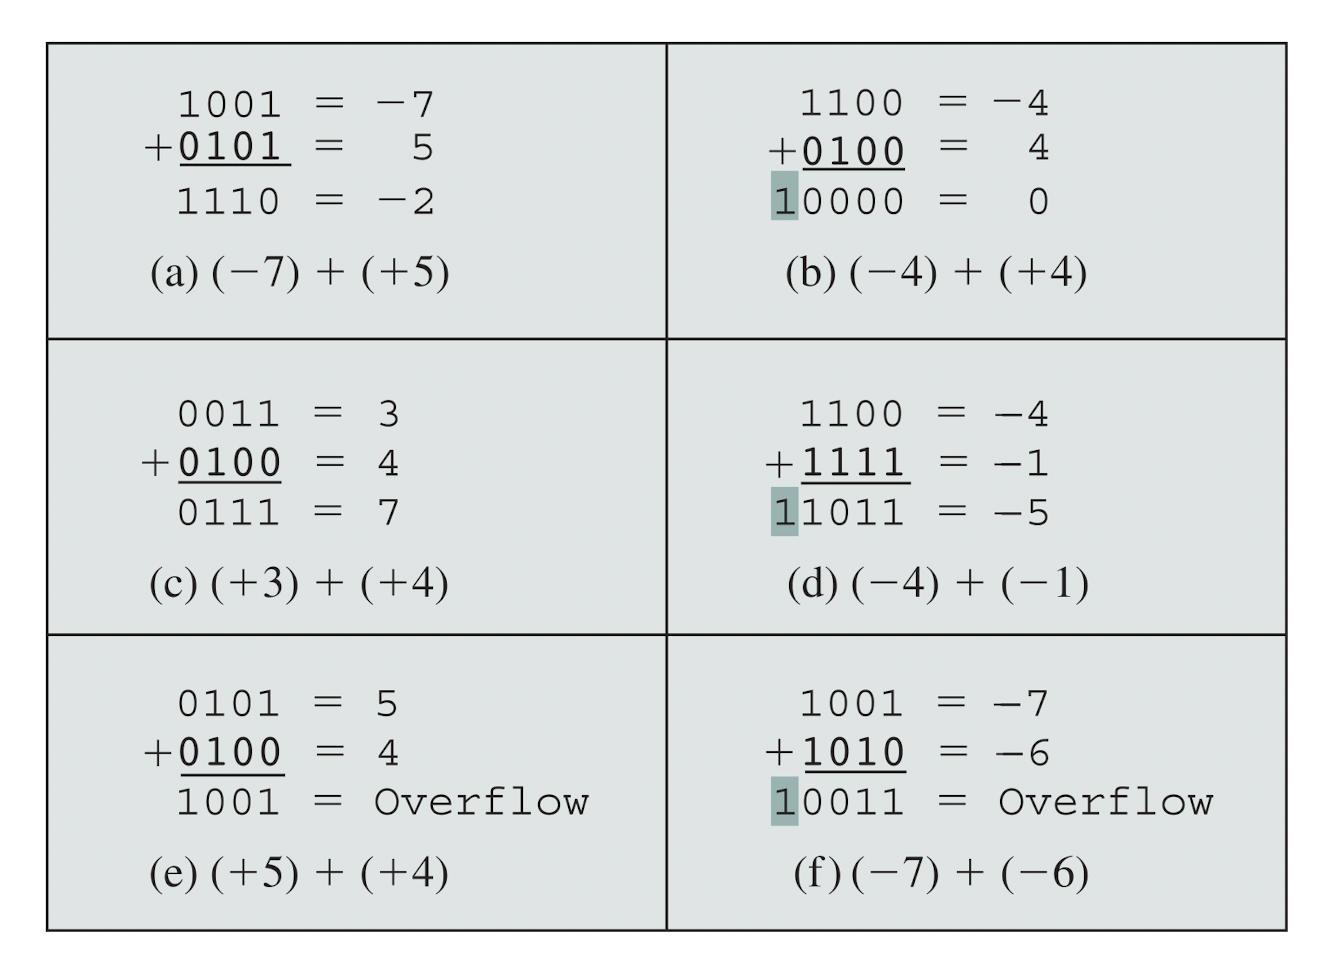
\includegraphics[scale=0.2]{immagini/somma}
	\caption{La somma nei computer}
\end{figure}

La sottrazione avviene come un'addizione in cui il secondo addendo è l'opposto del sottraendo; è effettuato il cambio di segno al secondo membro della sottrazione.

La seguente immagine aiuta a comprendere in quale modo i numeri sono rappresentati nel caso della rappresentazione complemento a due.

\begin{figure}[h]
	\centering
	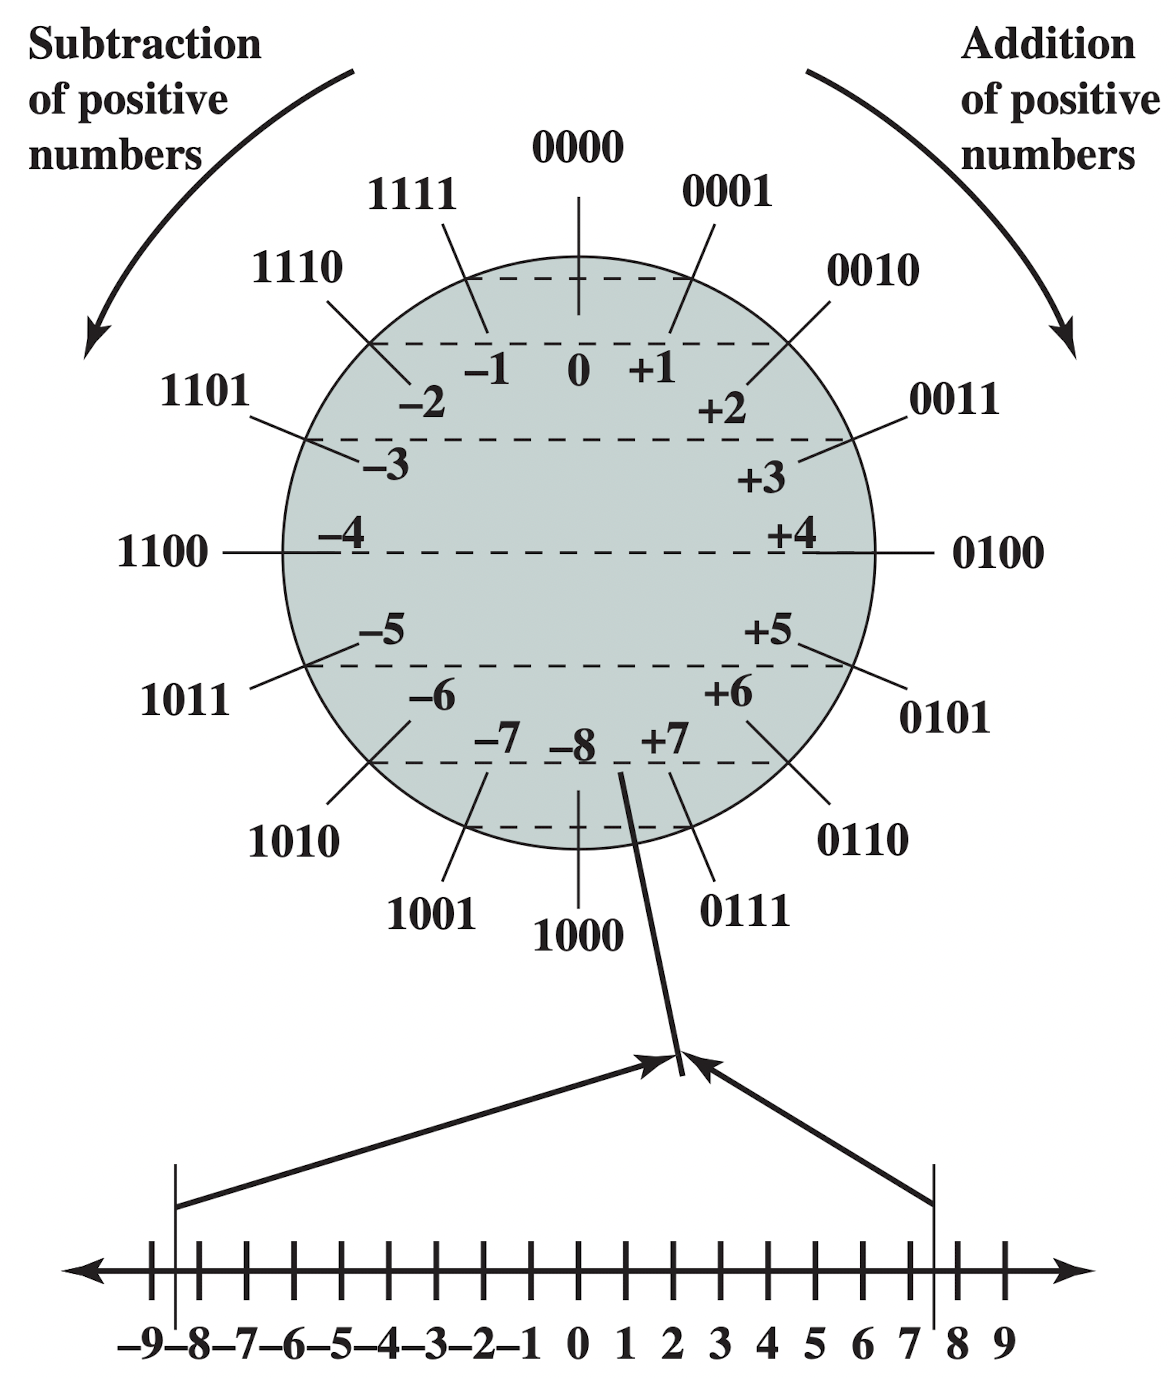
\includegraphics[scale=0.2]{immagini/complementoadue}
	\caption{Rappresentazione complemento a due; una parola vale 4 bit.}
\end{figure}

In questo caso l'\textit{overflow} si verifica quando addizionando o sottraendo si oltrepassa il punto finale in cui si trovano i limiti superiore ed inferiore.\\

Ora spieghiamo come viene effettuata un'addizione da un'ALU: gli addendi sono salvati ognuno in un registo; per semplicità li chiamiamo A e B; gli addendi sono prelevati dai registri e sono sommati, dopodichè il risultato è salvato o in un terzo registro oppure in uno dei due registri iniziali. Nel caso in cui si effettua una sottrazione, il sottraendo è prelevato dal suo registro, viene invertito il segno del numero e poi come prima è sommato ad all'altro addendo.

\subsubsection{La Moltiplicazione e la Divisione}
Rispetto all'addizione la moltiplicazione è un'operazione più complessa. In generale questa è l'idea dietro alla moltiplicazione:
\begin{enumerate}
	\item sono effettuate delle moltiplicazioni parziali e poi queste sono sommate;

	\item Se il moltiplicatore, che è composto da una sola cifra, è 1, allora il moltiplicando è riscritto, facendolo slittare di una posizione (come se venisse moltiplicato per 10, di fatto lo si moltiplica per 2); se il moltiplicatore è 0, allora non si fa nulla, semplicemente bisogna ricordarsi di far slittare il numero successivo di una posizione in più.
\end{enumerate}

Per ottimizzare questi passaggi si effettua una somma parziale mano a mano che si ottengono i risultati delle moltiplicazioni parziali; in questo modo si preserva spazio nei registri. In sostanza la moltiplicazione è composta da slittamenti di una posizine a destra e di somme. Poichè la moltiplicazione restituisce risultati che richiedono fino a due volte i bit necessati per rappresentare i fattori della moltiplicazione, il risultato è salvato tra il registro del primo fattore ed il registro del secondo fattore.\\
Infine bisogna effettuare uno xor, $\oplus$, dei segni dei fattori. Questo metodo si rivela essere piuttosto lento, per questo motivo si utilizza l'algoritmo di Booth.\\

La divisione è calcolata in modo simile: con gli slittamenti, addizioni e sottrazioni ripetute.

\subsection{I Numeri Razionali}

Poichè i computer possono utilizzare solo un numero finito di bit non sono in grado di rappresentare i numeri reali; per questo motivo si possono rappresentare solo alcuni numeri razionali, che sono chiamati \textit{float}. Il metodo per rapprestare questi numeri è denominto a virgola mobile ed è utilizzato per indicare sia numeri con la virgola che numeri molto grandi. In generale la parola (intesa come set di bit) utilizzata per rappresentare questi numeri è divisa in tre:
\begin{enumerate}
	\item Il primo numero rappresentato è il significando: è il numero più a sinistra ed è un un 1 od uno 0; in questo modo si possono rappresentare sia i numeri positivi che i numeri negativi. Con la rappresentazione a virgola mobile viene introsotta la base scientifica, il funzionamento è il medesimo. Per questo motivo c'è solamente una cifra con segno prima della virgola. L'1 rappresenta $-1$, mentre lo zero rappresenta $1$;

	\item \label{bias} come anticipato precedentemente, viene introdotta la notazione scientifica, per questo motivo la parte intermedia del \textit{float} rappresenta l'esponente. L'esponente può essere sia positivo che negativo; il medoto per rappresentare l'esponente è chiamato esponente polarizzato, praticamente i bit che indicano l'esponente si riferiscono ad un numero che poi viene sottratto per un altro numero n; n varia a seconda dell'architettura dei computer, in genrale $n=2^{k/2}-1$ dove $k$ è il numero di bit che sono utilizzati per rappresentare l'esponente. n è chiamato bias.

	\item \label{mantisse}Dopo la virgola è riportato un numero naturale che rappresenta il numero dopo la virgola;
\end{enumerate}

Come si può intuire non possono essere rappresentati tutti i numeri, ma solo quelli con un numero finito di cifre decimali. Inoltre esiste un numero massimo di numeri rappresentabile: come è ovvio che sia se i float sono caratterizzati da n bit, possono rappresentare solo $2^n$ numeri diversi, come è intuibile dalla formula per calcolare il valore massimo esprimibile in bit, \autoref{valoremassimo}.
In questo modo si possono verificare 4 tipi di \textit{overflow}, in base alla grandezza del numero da rappresentare. Nel qual caso si chieda di rappresentare un numero eccessivamente preciso, con troppe cifre significative il problema non si chiama \textit{overflow} e il numero è arrotondato al numero rappresentabile in virgola mobile più prossimo.

\subsubsection{Le quattro operazioni}
\paragraph{L'addizione e la sottrazione} nel caso dei \textit{float} è più complessa: per esempio è possibile sommare due numeri di ordine di grandezza diverso. Per questo motivo ci sono 4 fasi principali per svolgere le somme e le sottrazioni con questi numeri:
\begin{enumerate}
	\item prima di tutto i computer calcolano solo le addizioni. Per eseguire la sottrazione al minuendo si addiziona l'opposto del sottraendo;

	\item se il risultato può essere un'approssimazine della somma dei due float allora si compie l'allineamento della mantisse; praticamente si pongono gli zero dove è necessario per il numero più piccolo in modo tale che l'esponente sia il medesimo;

	\item viene effettuata l'operazione tra le due mantisse, \autoref{mantisse}, i due numeri senza l'esponente; è come se venisse applicata la priprietà associativa e il $2^k$ è preso come fattore comune.

	\item \label{normalizzazione}in conclusione si slitta il risultato a sinistra aumentando l'esponente di 1, $+1$, per ogni slittamento verso sinistra, oppure al contrario si slitta il risultato a destra e si sottra 1, $-1$ per ogni traslazione di una posizione. Ovviamente la mantisse ha un numero finito di cifre decimali, per questo motivo molte volte le operazioni con i \textit{float} sono approssimate. Questo passaggio è chiamato normalizzazione.
\end{enumerate}

\paragraph{La moltiplicazione e la divisione} sono processi più semplici, invece.
In questo caso ci sono 5 fasi per calcolare il risultato dell'operazione:
\begin{enumerate}
	\item all'inizio è fatto il controllo degli zeri ed è effettuato il rispettivo cambio del segno se necessario;

	\item dopodichè è effettutata la somma o la sottrazione tra gli esponenti ed è sottratto il bias, \autoref{bias}, poi si controlla che il risultato sia accettabile; cioè si controlla che il risultato non sia un \textit{overflow} oppure un \textit{underflow};

	\item viene effettuata l'operazione e quindi è calcolato il risultato;

	\item si normalizza il risultato, \autoref{normalizzazione} ed ancora una volta si controlla per eventuali \textit{overflow} oppure \textit{underflow};

	\item Infine il risultato viene approssimato in modo tale che possa essere scritto come \textit{float}: c'è un numero fissato di bit utilizzabile. Questo passaggio è chiamato arrotondamento.
\end{enumerate}

\section{Il linguaggio macchina}
In sostanza questa section spiega i processi che l'ALU compie per elaborare i dati. Quindi spieghiamo il ciclo di un'istruzione; bene o male approfondiamo quanto già visto, \autoref{cicloistruzione}. Innanzitutto, l'ALU ha l'indirizzo di un'istruzione, la quale contiene diverse informazioni:

\begin{itemize}

	\item l'operazione da eseguire,  per esempio add o sub o I/O, questa informazione è codificata in binario ed è chiamata codice operativo, opcode;

	\item il \textbf{riferimento} agli operandi;

	\item il \textbf{riferimento} in cui salvare il risultato dell'operazine;

	\item l'indirizzo della prossima istruzione, che può essere un indirizzo fisico o logico. In realtà un'istruzione contiene l'indirizzo di un'altra istruzione se viene effettuato un jump, altrimenti il \textit{program counter} si aggiorna e indica l'istruzione successiva;

\end{itemize}

Gli operandi sono salvati in una delle seguenti memorie:
\begin{itemize}
	\item nella memoria centrale o virtuale, nella RAM; in questo caso il riferimento è un indirizzo;

	\item in uno dei registri della CPU, che è identificato grazie ad un numero;

	\item nell'istruzione, il dato è contenuto direttamente dentro l'istruzione;

	\item in una periferica; in questo caso il riferimento è l'indirizzo dell'operando.
\end{itemize}

Un'istruzione è divisa in diversi campi: il campo codice operativo e uno o più campi indirizzo.
Il numero di indirizzi contenuti in un'istruzione varia a seconda dell'architettura; per esempio un operando può essere contenuto nell'accumulatore, per questo motivo anche se l'operazione è l'addizione è sufficiente il riferimento ad un solo operando;
Oppure è possibile che tutti gli indirizzi degli operandi siano impliciti; in questo caso è necessario che l'hardware sia dotato di una pila, una \textit{stack}.\\

Un tempo si preferiva un'architettura con indirizzi più brevi e quindi con operandi e istruzioni implicite; per questo motivo i programmi erano più lenti e più complessi. Oggi sono aumentati i registri delle CPU e dunque non c'è bisogno di indicare indirizzi interi, è sufficiente che l'istruzione contenga il numero che identifica il registro.\\

Un altro discorso interessante riguarda il set di istruzioni di cui dispone un PC: esistono due architetture molto distinte, la CISC e la RISC. Per intenderci la CISC, \textit{Complex Instruction Set Computer}, implementa nell'hardware il più grande numero di istruzioni possibile; per converso la RISC, \textit{Reduced Instruction Set Computer}, limita il set al minimo indispensabile. I computer moderni adottano una mezza via tra le due: la Apple è orientata verso la RISC, mentre l'Intel è più prossima alla CISC.

\subsection{Progettare un Set di Istruzioni}

Come abbiamo visto, in elaboratori diversi le istruzioni racchiudono i dati in modi peculiari: quando si progetta un computer bisogna pensare alle caratteristiche da dare ad un set di istruzioni. Risulta utile elencare le peculiarità che caratterizzano un set di istruzioni:
\begin{itemize}
	\item Repertorio operazionale: l'elenco delle operazioni eseguibili da in computer;

	\item Tipo di Dato: le classi disponibili nell'ALU (indirizzi, numeri (float, int), caratteri (chr, string), dati logici (True, False));

	\item Formato: le dimensioni dei campi ed i campi dell'istruzione;

	\item Registri: il numero dei registri disponibili all'ALU;

	\item Indirizzamento: la politica che si sceglie di adottare per indicare il riferimento degli operatori.
\end{itemize}

Per sfruttare i dati logici è necessario l'indirizzamento al byte.

\subsection{Metodi di Indirizzamento degli Operandi}

Ci sono molti metodi per indicare il riferimento degli operandi all'interno delle istruzioni.
\begin{itemize}
	\item \textbf{Indirizzamento Immediato}: l'operando è direttamente contenuro nell'istruzione; l'operando deve essere breve. 0 accessi in memoria;

	\item \textbf{Indirizzamento Diretto}: il campo indirizzo rimanda alla cella in memoria con l'operando; in questo caso l'indirizzo deve essere breve; 1 accesso in memoria;

	\item \textbf{Indirizzamento Indiretto}: il campo indirizzo  rimanda ad una cella in memoria che contiene l'indirizzo in cui si trova l'operando. Poichè il campo indirizzo è più corto degli indirizzi normalmente rappresentabili nei computer, con un indirizzo breve si rimanda ad una cella che contiene un indirizzo intero. 2 accessi in memoria;

	\item \textbf{Indirizzamento Registro}: il campo indirizzo rimanda ad un registro che contiene l'operando. Utilizzando questo metodo, il campo indirizzo è breve, inoltre la risposta da parte dei registri è molto veloce. 0 accessi in memoria;

	\item \textbf{Indirizzamento Registro Indiretto}: il campo indirizzo punta ad un registro che contiene un indirizzo che rimanda all'operando;

	\item \textbf{Indirizzamento con Spiazzamento} \label{spiazzamento}: il campo indirizzo si divide in due, A (address) e R (register). L'indirizzo R rimanda ad un registro che contiene un puntatore. Questo indirizzo è sommato all'indirizzo A per ottenere l'indirizzo della cella di memoria con l'operando. Di seguito sono elencati i metodi per effettuare l'indirizzamento con spiazzamento.

	\begin{enumerate}
		\item \textbf{Indirizzamento Relativo}: in questo caso R rimanda al \textit{program counter}, \autoref{programcounter}. All'indirizzo ivi contenuto è sommato il valore A. 0 o 1 accesso in memoria;

		\item \textbf{Indirizzamento Registro-Base} \label{registrobase}: R contiene un puntatore che indica un'area della memoria, a questo indirizzo è aggiunto l'indirizzo A per ottenere l'indirizzo dell'informazione che interessa. 1 accesso in memoria;

		\item \textbf{Indicizzazione}: In questo caso vengono estratti molti operandi: a partire da un indirizzo A, che chiamiamo base, estraiamo tutti i dati delle celle di memoria successive. A indica l'indirizzo base ed in R è memorizzato un valore che viene sommato per estrarre il dato utile. A viene nuovamente addizionato ad R e si estrae il dato successivo. In questo modo sono estratti più dati, fino al termine dell'array che li contiene. diversi accessi in memoria;

	\end{enumerate}

	\item \textbf{Pila}: il campo indirizzo è vuoto: l'operando o gli operandi necessari sono in cima alla pila; lo \textit{stack pointer} indica la cima della pila. Grazie al comando pop(), il programmatore può estrarre il dato in cima;
\end{itemize}

Ogni computer sfrutta più di un metodo; ma allora un PC come conosce che metodo sta venedo applicato? Senz'altro il codice operativo aiuta i computer ad intuire il metodo sfruttato; in aggiunta, un'istruzione può essere composta dal \textit{mode field}, un campo dell'istruzione che contiene qualche bit e serve per indicare il metodo utilizzato.

\subsection{Il Formato delle Istruzioni}

Il formato delle istruzioni riguarda i campi campi di un'istruzione e la quantità di bit che ciascun bit richiede. Tutte le istruzioni sono dotate del campo codice operativo, ma a seconda dell'operazione svolta servono più o meno bit. Per esempio svuotare l'accumulatore non richiede operandi oppure riferimenti alla memoria. Uno store richiede i dati in una specifica cella di memoria e il riferimento al registro in cui salvare i bit. La lunghezza delle istruzioni richiede uno studio attento, perché ha diverse implicazioni sulle caratteristiche organizzative dei computer.

\subsubsection{La Lunghezza delle Istruzioni}

I computer sono progettati in modo tale da aiutare il lavoro dei programmatori, per questo motivo si effettua uno studio attento sulla lunghezza delle istuzioni; idillicamente si vuole avere un computer con un set di istuzioni molto ampio, molti metodi di indirizzamento e molti registri in cui salvare i dati. Tutto ciò è possibile solamente aumentando le dimensioni delle istruzioni; tuttavia, utilizzando istruzioni lunghe si rischia di rallentare l'accesso in memoria a tal punto che il processore finisce di svolgere le istruzioni prima che sia completo il fetch delle successive. Come spiegato alla \autoref{microprogrammazione}, bisogna fare in modo che tutte le componenti lavorino nello stesso momento per ottimizzare il tempo. Per questo motivo si tenta di individuare il giusto compromesso tra lunghezza delle istruzioni e semplicità di programmazione: in 32 bit stanno due istruzioni da 16 bit che impiegano più tempo ad essere svolte di un'unica istruzione a 32 bit.\\
In aggiunta è necessario che i bit di un'istruzione siano un multiplo di parola o il contrario; in modo tale da permettere il \textit{fetch} delle istruzioni in una volta unica oppure in un numero di volte ben definito, senza trovarsi con mezze istruzioni, che a loro volta richiederebbero altri \textit{fetch}.

\subsubsection{Asseganzione dei Bit}

Allo stesso modo è importante identificare la quantità di bit che sono disponibili per definire il codice operativo. Un codice operativo che conta molti bit rischia di allungare eccessivamente le istruzioni, per cui il fetch diventa molto lento; d'altro canto molte operazioni sono uniche e sono necessarie per cui hanno bisogno di una codifica in bit. Un codice operativo di $n$ bit identifica fino a $2^n$ operazioni diverse. Se la lunghezza del campo opcode è fissata le operazioni che richiedono molti operandi utilizzano metodi di indirizzamento concisi, ma lenti, come l'indicizzazione.

Poichè i bit di un'istruzione sono così importanti analiziamo le cause che occupano i bit:
\begin{itemize}
	\item \textbf{Numero di metodi di indirizzamento}:  Alcune istruzioni hanno bisogno di specificare quale metodo di indirizzamento viene utilizzato, per questa ragione sono necessari da uno a due bit; (conteggio 2)

	\item \textbf{Numero di Operandi}: un'istruzione richiede bene o male due operandi ed ognuno richiede richiede di esemplificare il proprio metodo di indirizzamento; (conteggio 4)

	\item \textbf{Registri}: i registri aiutano molto: diminuiscono gli accessi in memoria, inoltre solo circa 32 registri sono indirizzabili dal programmatore; in questo modo un dato salvato nei registri richiede al massimo 5 bit. Dopo tanti tentativi si è notato che più di 32 registri rallentano il PC; (conteggio 7)

	\item \textbf{Numero di Set di Registri}: nei computer sono montati registri specializzati in base all'utilizzo; il set di registri da leggere è determinato in base al codice operativo. In ogni set ci sono circa 32 registri, ma ci sono più set, in questo modo sono sufficienti 5 bit per indicare l'indirizzo; (conteggio 7)

	\item \textbf{Intervallo di Indirizzi}: il campo indirizzo non permette di indicare qualunque indirizzo in memoria, per questo motivo è sfruttato l'indirizzamento a spiazzamento, \autoref{spiazzamento};

	\item \textbf{Granularità degli Indirizzi}: l'indirizzamento al byte richiede un numero maggiore di bit, per questo motivo può essere sconveniente; d'altro canto, manipola i dati accuratamente.
\end{itemize}

\section{Esempi di Architetture Passate}
\subsection{PDP-8}

Il PDP-8 sfruttta un'architettura a 12 bit, dalla posizione 0 alla 2 è indicato l'opcode, tuttavia nel caso in cui opcode sia $hex7$, allora il resto dell'istruzione codifica delle microistruzioni, che non necessitano di operandi (per esempio, svuota l'accumulatore). In questo modo, il PDP-8 è in grado di effettuare circa 35 istruzioni. Si dice che la lunghezza delle istruzioni è fissa, ma il formato è variabile, infatti ci sono due possibili formati: da una parte ci sono tutte le operazioni che hanno bisogno degli operandi, dall'altro i dodici bit codificano solo operazioni, senza alcun riferimento alla memoria o dati immediati.

\subsection{PDP-10}

L'hardware è molto complesso per rispettare tre proprietà delle istruzioni:
\begin{itemize}
	\item Ortogonalità: l'indirizzo non è mai implicito, non dipende dal codice operativo;

	\item Completezza: sono utilizzate le medesime istruzioni per eseguire calcoli algebrici su tutte le classi numeriche (float, int, fixed-point);

	\item Indirizzamento Diretto: l'indirizzo è sempre esplicito ed è indicato nelle istruzioni (aiuta molto i programmatori).
\end{itemize}

La \textit{word} conta 36 bit, per questo motivo anche le istruzioni sono lunghe 36 bit. Il campo codice operativo misura 9 bit. Con 9 bit è possibile effettuare $2^{9}=512$ operazioni diverse; in realtà in questa architettura esistono 356 operazioni. Le operazioni in genere richiedono 2 operandi, il primo si trova in un registro generale, che per essere indicato richiede 4 bit, dunque avanzano 18 bit per indicare l'indirizzo del secondo operando. In questo modo si può utilizzare l'indirizzamento immediato, per cui il dato è direttamente contenuto nell'istruzione; altrimenti è bene utilizzare l'indirizzamento diretto, per cui si effettua un accesso in memoria; in base all'istruzione sono utilizzati anche indirizzamento indiretto (registro se possibile), e l'indicizzazione. Con questa architettura si sacrificano le prestazioni, ma la programmazione diventa molto semplice sia per il programmatore che per il compilatore. Infatti c'è uno spreco sulla quantità delle informazioni condivise. Si dice che le istruzioni hanno lunghezza fissa e c'è un solo formato.\\

Esistono anche architetture che sfruttano istruzioni a lunghezza variabile; poichè le istruzioni possono avere lunghezze diverse, quando si importa un'istruzine si recuperano tanti bit quanti ne prevede la l'istruzione più lunga; in questo modo il PC è sicuro di avere fatto il \textit{fetch} completo dell'istruzione successiva.

\subsection{PDP-11}

Nel formato delle istruzioni PDP-11, una parola è lunga 16 bit e le istruzioni misurano una parola; tuttavia, per aumentare la flessibilità e la compattezza dei dati condivisi, è possibile scrivere istruzioni lunghe 32 o 48 bit. Questo formato gode della proprietà ortogonale, grazie alla quale il metodo di indirizzamento è indipendente dal condice operativo, in questo modo è possibile utilizzare qualunque metodo di indirizzamento con tutte le operazioni. Con il formato PDP-11, è presente un set da otto registri ad uso generale. Due di questi registi sono il \textit{program counter}, \autoref{programcounter}, che contiene l'indirizzo della prossima istruzione; ed lo \textit{stack pointer}. In sostanza, grazie a questo formato, il set delle istruzioni ed i metodi di indirizzamento sono molto complessi, ma i programmi sono compatti ed efficienti. Si dice che le istruzioni hanno lunghezza variabile e ci sono 13 formati diversi.

\subsection{VEX}

Anche in questo formato delle istruzioni, VEX, le istruzioni hanno lunghezza variabile; per quanto la maggior parte delle istruzioni necessitino solamente 1 byte e quindi 8 bit, alcune istruzioni misurano 37 byte. Il set di questo formato conta circa 300 istruzioni che non sono rappresentabili da 8 bit, per questo motivo nel qual caso il primo byte sia in esadecimale FD o FF, è eseguito il \textit{fetch} dei 2 byte successivi, dove è specificato il codice operativo. Il campo per riferire un operando varia dal singolo byte, in cui i 4 bit più a sinistra spiegano il metodo di indirizzamento; ad eccezione di un segnale in cui i due bit significativi non siano 00, in questo caso si utilizza l'indirizzamento diretto.
Di solito il riferimento di un operando consiste in un byte in cui le 4 cifre più a destra puntano ad un registro ($2^4= 16$ registri ad uso generale).

%non ho compreso in quale modo si riesce ad incrementare le dimensioni delle istruzioni, dovrei chiedere a Leo.

\subsection{Il Formato delle Istruzione x86}

Il formato delle istruzioni x86 è molto flessibile e compatto, ci sono molti metodi diversi per indirizzare gli operandi e il codice operativo ha lunghezza variabile.

\begin{figure}[h]
	\centering
	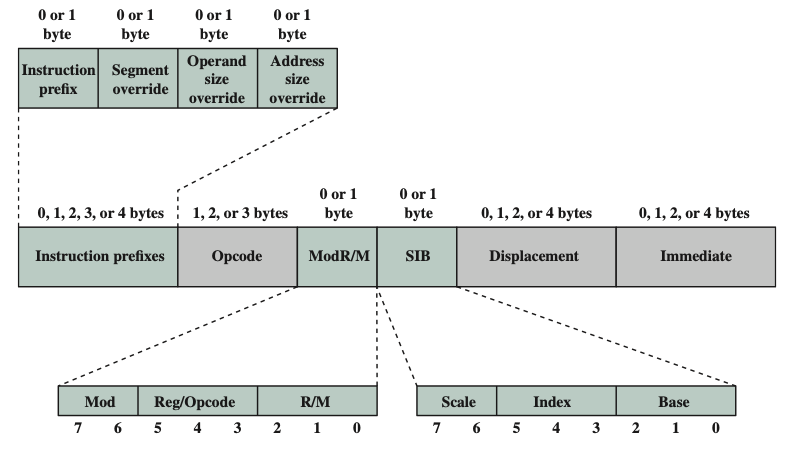
\includegraphics[scale=0.3]{immagini/formatox86}
	\caption{I campi che potrebbe avere un'istruzione nel formato x86.}
	\label{formatox86}
\end{figure}

In questo formato, come si deduce dall'immagine esemplificatica \autoref{formatox86}, solamente il campo codice operativo è sempre presente. Ora risulta necessario esemplificare l'immagine:
\begin{enumerate}

\item I primi byte dell'istruzione:
\begin{enumerate}
	\item \textbf{prefisso dell'istruzione}: può essere LOCK prefix, per cui si indica alla memoria di non condividere con gli altri core gli operandi prelevati; in alternativa, si tratta di un prefisso di ripetizione, che indica in quale modo una determinata operazione deve essere ripetuta;

	\item \textbf{segment override}: viene specificato il registro in cui salvare le informazioni per salvare la base nell'indirizzamento registro-base (registrobase);

	\item \textbf{operand size}: un operazione implicitamente è accompagnata da operatori da 16 o 32 bit, questo prefisso indica l'altra lunghezza;

	\item \textbf{address size}: come il caso dell'operand size, caso precedente (si switcha tra 16 e 32 bit, rispetto alla lunghezza dell'indirizzo data un'operazione).
\end{enumerate}

\item Il codice operativo: la lunghezza di questo campo varia tra il byte ed i tre byte. All'interno di questa sezione dell'istruzione viene specificata la lunghezza dei dati, 16 o 32 bit (sembrerebbe contraddirsi con operand size) o se c'è bisogno di più byte per un indirizzamento immediato;

\item ModeR/M: questo byte indica se l'operando è salvato in memoria (M) oppure in un registro (R); in aggiunta, specifica il metodo di indirizamento utilizzato, ove necessario l'indicizzazione. Ci sono tre bit per specificare l'operazione o il registro;

\item SIB: ogni tanto ModeR/M potrebbe non contenere abbastanza informazioni, in questo caso i dati in più sono comunicati qui;

\item Spazzamento: se è utilizzato questo metodo di indirizzamento degli operandi, viene aggiunto questo campo per indicare il riferimento;

\item Immediato: se è utilizzato questo metodo di indirizzamento, qui viene inserito l'operando.
\end{enumerate}

Come si evince dalla spiegazione qui sopra riportata, il formato x86 è molto flessibile: permette di indicare il riferimento di un operando in molti modi diversi, però si riesce a specificare solo un operando per operazione. D'altro canto si riescono ad estrarre molti dati da un array posizionato ovunque nella memoria, praticamente non esiste limite ai dati estraibili con l'indicizzazione. Questo formato è stato pensato per essere compatibile con macchine più vecchie e per venire in contro alle richieste dei designers. Con questo formato si riesce a scrivere del codice molto efficiente.

%sarebbe bello recuperare la pagina 503, descrive l'evoluzione dei formati nei computer con architettura ARM.

\section{La Struttura interna del Processore}

Come abbiamo approfondito nel ciclo di un'istruzione \ref{cicloistruzione}, la CPU deve svolgere determinati passi per completare un'istruzione: \textit{fetch} dell'istruzione, decondifica dell'istruzione, \textit{fetch} dei dati, elaborazione dei dati e scrittura dei dati. In questo capitolo approfondiamo questo ciclo.\\
Un processore è organizzato in questo modo:

\begin{figure}[h]
	\label{processore}
	\centering
	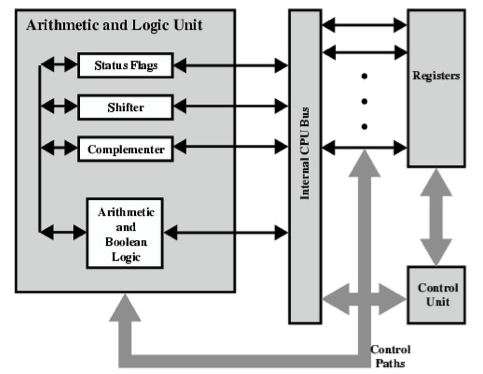
\includegraphics[scale=0.3]{immagini/processore}
	\caption{La struttura interna di un processore.}
\end{figure}

L'ALU elabora i dati, l'unità di controllo gestisce i dati in entrata ed il movimento dei dati all'interno del processore e controlla le operazioni che sono svolte dall'ALU. Ricordo che il bus interno è il dispositivo che permette la comunicazione tra le componenti della CPU.

\subsection{I Registri Utente}

I registri nel processore sono memorie veloci, piccole e costose. Nella CPU i registri sono  in due categorie:
\begin{itemize}
	\item \textbf{Registri Utente}: accessibili al programmatore, diminuiscono gli accessi in memoria;

	\item \textbf{Registri di Controllo e di Stato}: accessibili alla CU (\textit{control unit}) per controllare l'ALU; anche il sistema operativo può accedervi.
\end{itemize}

In realtà la distinzione in queste due categorie varia a seconda dell'architettura degli elaboratori. (Un programma in assembler è tradotto in codice macchina, binario, dall'assemblatore, +linker )\\

I registri utente sono a loro volta divisi in quattro categorie:
\begin{itemize}
	\item Ad uso generale;

	\item Dati: si tratta di registri \textit{ad hoc} per contenere operandi. Possono essere divisi in base alla classe di dati che contengono o in base all'operazione che li chiama;

	\item Indirizzi: contengono indirizzi (indirizzamento registro-base, indicizzazione, pila, \autoref{registrobase});

	\item Codici di Condizione: fino ad ora ci siamo riferiti ai codici di condizione con il nome \textit{flag}; abbiamo trovato questi bit nel caso di \textit{overflow}. Un altro utilizzo di queste memorie è il caso delle condizioni, non è detto che i registri possano essere toccati dal programmatore (comuque questo punto è solamente enunciato; in aggiunta non sono pochi gli svantaggi di questa tecnologia);
\end{itemize}

In alcune architetture questa divisione non è manichea: i registri Dati e Indirizzi non sono divisi; questo ha dei pro e dei contro. La divisione dei registri riduce la flessibilità del programmatore. D'altro canto, unire le due tipologie di registro genera i propri disagi: a parità di registri sono necessati più bit per indicare il registro; il registro dati potrebbe essere più capace di quello indirizzi, quindi bisognerebbe occupare due registri indirizzi per salvare un dato, oppure se si salva un indirizzo nei registri dati viene sprecata una porzione della memoria. La tecnologia RISC utilizza un approccio diverso sotto questo punto di vista.

\subsection{I Registri di Controllo di Stato}

I registri di controllo di stato variano molto in numero e in specializzazione, di seguito sono riportati i registri essenziali:
\begin{itemize}
	\item \textbf{program counter}: contiene l'indirizzo dell'istruzione che deve ancora essere recuperata;

	\item \textbf{instruction register}: contiene l'ultima istruzione prelevata;

	\item \textbf{memory address register}: contiene l'indirizzo di una cella di memoria;

	\item \textbf{memory buffer register}: contiene una \textit{word} di dati che deve essere scritta in memoria oppure la \textit{word} dato dell'ultimo dato estratto.
\end{itemize}

Il processore aggiorna il \textit{program counter} ogni volta che un'istruzione è prelevata dalla memoria, oppure quando viene effettuata una brench oppure una skip instruction.
Dopo aver eseguito il \textit{fetch} l'istruzione è mandata nell'IR dove è analizzata. L'indirizzo degli operandi è calcolato utilizzando il MAR, che inoltra l'indirizzo direttamente al bus di sistema; poi il dato arriva nell'MBR attraverso il bus.\\

In aggiunta, esiste un altro registro chiamato \textit{program status word}, che immagazzina diversi dati:
\begin{itemize}
	\item segno dell'ultimo risultato;

	\item zero;

	\item riporto;

	\item uguale;

	\item overflow;

	\item abilitazione o disabilitazione dell'interrupt;

	\item supervisore: tiene contro delle autorizzazioni delle istruzioni che sono svolte.
\end{itemize}
Ognuno di questi dati è contenuto in un bit, in totale questo registro contiene 7 bit.

\section{La \textit{Pipeline}}\label{pipeline}

\subsection{Il ciclo di \textit{fetch}}

Avendo l'indirizzo di un'istruzione viene eseguito il \textit{fetch} dell'istruzione: l'indirizzo è spostato nel MAR, che ha accesso diretto con il bus. La memoria manda indietro i contenuti nella locazione indicata e l'istruzione arriva all'MBR e poi è spostata nell'IR.
Nell'IR l'istruzione è analizzata. Ove necessario un altro \textit{fetch}, la porzione di istruzione è rimandato al MAR ed i dati sono inviati dallo storage all'MBR. Notare che se l'indirizzamento è indiretto, allora il dato ricevuto dall'MBR è rimandato al MAR per eseguire un ulteriore ciclo di \textit{fetch}.\\
Nel qual caso si verifichi un'interruzione, il contenuto del PC è copiato nell'MBR; mentre lo \textit{stack pointer} o un altro indirizzo di locazione di memoria speciale è caricato nel MAR. Poi si ricomincia da capo con il \textit{fetch} dell'istruzione. L'interruzione è condivisa dalla UC.\\
Dal momento che il \textit{fetch} di un'istruzione o degli operandi e l'elaborazione dati utilizzano risorse differenti, è possibile eseguire il \textit{fetch} dell'istruzione successiva mentre viene eseguita la prima istruzione; questo processo è chiamato prefetch. La fase di \textit{fetch} molto spesso è più veloce rispetto all'esecuzione dell'istruzione, per cui si risparmia del tempo, ma alcune risorse sono sprecate; in aggiunta, sono frequenti le interruzioni oppure i brench o i salti (skip o jump) che si traducono in un \textit{discard}: l'IR viene riscritto, di fatto rendendo inutile il \textit{prefetch}. Per questo motivo è introdotta la pipeline, una catena di montaggio, fondamentalmente. \\
Dal momento che il \textit{fetch} di un'istruzione è più veloce dell'esecuzione di un'istruzione, si divide il ciclo di esecuzione di un'istruzione in più fasi possibili ed in fasi della medesima durata. Nel momento in cui un componente finisce il proprio lavoro invia gli output al componente successivo che deve essere pronto a riceverli. Dal momento che una sincronizzazione fino a questo livello non è possibile sono introdotti dei registri che memorizzano tutti gli output di un componente. I buffer sono piccoli, quindi non riescono ad immagazzinare più di un output per volta, per questo motivo, una volta che si divide il ciclo di esecuzione di un'istruzione in più fasi, è importante che tutte le fasi siano sempre sincronizzate (altrimenti i dati sono sovrascritti e persi). \\
Nei computer moderni la \textit{pipeline} è divisa in 24 stage diversi; dal momento che l'implementazione hardware e la progettazione diventano complesse aumentando le fasi della \textit{pipeline}, oggi si sono aumentati i core, introducendo il parallelismo di fatto. \\

La pipeline ha tre problemi principali:
\begin{itemize}
	\item \textbf{non tutte le fasi hanno la medesima durata} e abbiamo chiarito l'importanza della sincronizzazione. Per questo motivo sono introdotte delle pause tra i vari stage, in questo modo il problema è arginato, ma non risolto;

	\item \textbf{non tutte le istruzioni hanno le medesime fasi}. Basti pensare che alcune istruzioni non hanno bisogno di alcun dato, per cui il \textit{fetch} degli operandi non è eseguito, questo vuol dire che la \textit{pipeline}, in qualche modo non rende tutte le istruzioni più veloci;

	\item \textbf{gli operandi possono dipendere da istruzioni ancora in esecuzione}. In fase di esecuzione di un programma, le istruzioni sono riordinate in modo da alternare istruzioni dipendenti con istruzioni non dipendenti; se questo non è possibile sono introdotte delle pause forzate;

	\item \textbf{non è possibile eseguire il \textit{fetch} dalla memoria nello stesso momento}. Per cui se bisogna recuperare l'istruzione dalla memoria e gli operandi sono riferiti direttamente o indirettamente, allora bisogna stabilire delle priorità. Questo problema è risolto posticipando il \textit{fetch} degli operandi; oppure le \textit{cache} sono divise in base ai dati che contengono, per quanto si diminuisca la flessibilità dell'architettuara; si noti che comunque non è divisa la memoria centrale, per cui il problema, ancora una volta è arginato e non risolto;

	\item \textbf{ci possono essere salti, interruzioni}, vedremo le possibili soluzioni.
\end{itemize}

Per i motivi qui sopra riportati, la \textit{pipeline} migliora le prestazioni, ma non quanto ci si potrebbe aspettare.\\
Per calcolare lo \textit{speedup}, il fattore di taglio delle tempistiche, viene calcolato nel seguente modo:
\begin{equation}
	S_k=\frac{T_L}{T_k}=\frac{n\cdot k \cdot \tau}{(k+n-1)\cdot \tau}=\frac{n \cdot k }{n+k}
\end{equation}

In realtà, questo calcolo risulta vero solo nel momento in cui i problemi sopra citati non sono considerati.

\subsection{Le Dipendenza dai Dati}

Molte volte, le istruzioni che compongono un programma sono dipendenti l'una dall'altra, per esempio per effettuare un'addizione tra due operandi, bisogna prima caricare i dati nei registri del processore. Per arginare questo problema possono essere presi diversi provvedimenti:
\begin{itemize}
	\item \textbf{nop-stallo}: sono introdotte delle fasi non operative. Fino a che non sono disponibili gli operandi richiesti, l'istruzione che li chiama e le successive sono messe in pausa;

	\item \textbf{data forwarding}: non appena il dato è ottenuto, è passato direttamente all'istruzione successiva durante la fase di \textit{fetch} degli operandi oppure sono inoltrati direttamente all'ALU;

	\item \textbf{riordino delle istruzioni}: all'interno di un programma sono ricercate le istruzioni dipendenti e sono distanziate, in modo tale da non rallentare la pipeline, in figura \ref{riordinoistruzioni} è mostrato uno \textit{specimen} della soluzione;
\end{itemize}

\begin{figure}[h]
	\centering
	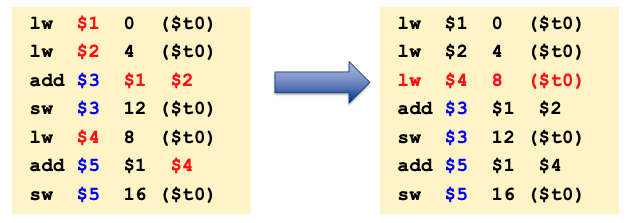
\includegraphics[scale=0.3]{immagini/riordinoistruzioni}
	\caption{Esempio di riordino delle istruzioni, in modo tale da ottimizzare la pipeline.}
	\label{riordinoistruzioni}
\end{figure}

\subsection{Le Dipendenze dal Controllo}

Le dipendenze dal controllo considerano tutti quei casi in cui un'istruzione prevede un salto, uno skip o un brench (lo skip salta solamente l'istruzione successiva, se vogliamo è un piccolo salto). Un salto è possibile nel caso in cui si utilizzi un ciclo for oppure un ciclo while; in questi casi viene effettuato un backflip: si torna indietro. Il brench è un modo diverso per riferirsi ad if, else, elif; se vogliamo il brench è anche try-except. Ci sono diverse soluzioni a questa problematica, prima fra tutte: ignorare il problema e bloccare il ciclo di esecuzione di un'istruzione nel momento in cui ci si accorge della possibilità del salto. Questa soluzione è poco pratica ed è sempre la più lenta.
Altrimenti si può scegliere di implementare un hardware con un'apposita logica di controllo.

\begin{itemize}
	\item Si può implementare un hardware che esegue il \textit{fetch} delle istruzioni in modo alternato tra le istruzioni successive a quella che indica il salto, e le istruzioni dopo l'istruzione target. In questo modo, in termini di probabilità non si guadagna nulla (sempre e solo metà delle istruzioni sono giuste, statisticamente parlando, sarebbe lo stesso se si ignorasse il salto). In questo caso un parte della pipeline è scartata.

	\item buffer circolare (\textit{loop buffer}) \label{loopbuffer}: in questo caso è implementato un buffer che funziona come una pila che contiene le istruzioni; di fatto il PC, \autoref{programcounter}, è lo \textit{stack pointer} di questa pila. Nel momento in cui è eseguito un salto di qualche tipo, si scorrono i tag delle istruzioni nella pila. Si verifica che il target non sia già presente nella pila; se l'istruzione target è già presente nella pila non c'è bisogno di eseguire un ulteriore \textit{fetch};

	\item predizione dei salti: viene associato qualche bit all'istruzione di salto, per prevedere se il salto avviene oppure no. In partiolare se viene associato un solo bit, si tiene conto dell'utltima volta che è stato eseguito un salto: se un'istruzione ha effettuato un salto il bit sarà impostato su 1 e quindi si eseguono le istruzioni a partire dall'istruzione target; altrimenti il bit avrà valore 0 e si ignora la possibilità di salto. \\
	Se i bit associati sono due esistono quattro possibilità:
	\begin{itemize}
		\item 10 $\rightarrow$ sono eseguite le istruzioni come se il salto venisse assolutamente preso. Se il salto non è preso allora i bit diventano 11;

		\item 11 $\rightarrow$ sono eseguite le istruzioni come se il salto venisse assolutamente preso. Se il salto è preso si torna al valore 10, se il salto non è preso i bit assegnati diventano 00;

		\item 00 $\rightarrow$ sono eseguite le istruzioni come se il salto non venisse assolutamente preso. Se il salto è preso allora i bit diventano 01;

		\item 01 $\rightarrow$ sono eseguite le istruzioni come se il salto non venisse assolutamente preso. Se il salto non è preso si torna al valore 00, se il salto è preso i bit assegnati diventano 10;
	\end{itemize}

	\item salto ritardato (\textit{delayed branch}): quando si trova un'istruzione di salto, si eseguono istruzioni che non hanno a che fare con il brench, fino a che il salto è eseguito o ignorato. Le istruzioni eseguite nel \textit{delay slot} potrebbero non essere utili.
\end{itemize}

\section{RISC}

Nel 2017 John L. Hennessy and David A. Patterson hanno ricevuto il Turing Award, il nobel dell'informatica, per aver introdotto uno studio sistematico e analitico alla progettazione dell'hardware dei computer. In particolare, Hennessy e Patterson hanno anticipato l'architettura RISC, \textit{Reduced Instruction Set Computer}.\\ Fondamentalmente, i due ricercatori statunitensi hanno analizzato la struttura dei programmi compilati in assembler ed il loro funzionamento. Hanno notato che ci sono dei processi molto frequenti: \textit{if} per C e l'\textit{assign} per pascal. Da questo studio hanno dedotto che un hardware migliore dovesse ottimizzare le operazioni più frequenti, piuttosto che implementare nell'hardware operazioni più complesse.
In particolare dalle ricerche degli anni `80 si ottengono alcuni dati utili ad ottimizzare la struttura hardware e software:
\begin{itemize}
	\item le operazioni più frequentemente usate sono di \textit{assign} e \textit{if};

	\item la maggior parte del tempo speso nell'esecuzione di un programma consta nel recupero di dati dalla memoria, sia dalle RAM che dalla cache;

	\item il 98\% delle funzioni (\textit{main}) utilizza meno di 6 procedure e il 92\% di ciscuna richiede meno di 6 operandi;

	\item la pipeline è inefficacie: molte delle istruzioni recuperate, sono scartate a causa di brench e \textit{loop}.
\end{itemize}

%1
Questi dati si traducono in un cambiamento radicale all'architettura, che all'epoca era CISC. L'architettura CISC comprende una vastissima gamma di opzioni per tradurre la stessa operazione; queste ricerche evidenziano che il grande numero di operazioni diverse comporta l'implementazione di un hardware di decondifica del codice operazionale, che rallenta molto il calcolatore. Per questo motivo, le aziende che producono i processori hanno progettato un'architettura RISC che mantenesse solo le operazioni più frequentemente usate; tale architettura comporta un taglio delle operazioni implementate, in quanto le operazioni meno frequenti sono svolte attraverso una sequenza di operazioni frequenti. Il numero ridotto di operazioni permette un'implementazione hardware che automaticamente aziona l'esecuzione di un'operazione, senza il bisogno di un processo di decodifica del codice operativo; questo taglio ha permesso di salvare un grande quantitativo di tempo. In realtà i PC prodotti oggi sono un mix tra le due architetture.\\
Non solo, la semplificazione del set di istruzioni permette di assemblare un hardware più lineare e compatto, quindi più prestante; il focus degli ingegneri cambia: ricercano metodi nuovi per ottimizzare il tempo di esecuzione delle operazioni strettamente necessarie. In questo modo gli indirizzi sono ridotti: sono necessari meno bit per indicare le operazioni.\\
%2

In aggiunta, si nota che gli accessi in memoria richiedono molto tempo, per questo motivo Intel \& co. hanno aumentato il numero di registri presenti nei processori. Grazie alla tecnologia RISC è stato ottimizzato l'utilizzo dei registri: un'operazione in genere necessita di tre registri: il registro dei parametri, il registro dei dati locali ed il registro dei dati temporanei; per questo motivo sono associti tre registri ad ogni operazione, questo gruppo di registri è chiamato finestra; molte volte in una procedura ne richiama un'altra, in genere ce ne sono 6 annidate; tendenzialmente le procedure annidate hanno bisogno di leggere i dati di uno dei registri della finestra della prima procedura; il registro dei dati temporanei di una procedura coincide con il registro dei parametri della procedura ad essa annidata.\\
%3

Dal punto di vista statistico, una funzione (una serie di funzioni è chiamato programma) non richiede un annidamento superiore a 6 livelli, per cui una finestra di 3 registri è collegata ad altre 5 finestre di tre registri, aventi ciascuna un registro in comune con la precedente; in totale una funzione richiede l'uso di 13 registri. Il metodo con cui sono assegnati i registri è scelto a livello hardware (è molto veloce!). Se una funzione richiede un annidamento superiore alle 6 operazioni i primi livelli sono portati in memoria. Il sistema utilizzato ricorda quello del buffer circolare (\textbf{loop buffer}, \autoref{loopbuffer}). La figura \ref{procedureannidate} esemplifica la connessione tra le finestre. Il core può accedere solamente ad una finestra per volta; quando è chiamata una procedura annidata il CWP, il puntatore che indica la finestra a cui è possibile accedere, cambia automaticamente.

\begin{figure}[h]
	\centering
	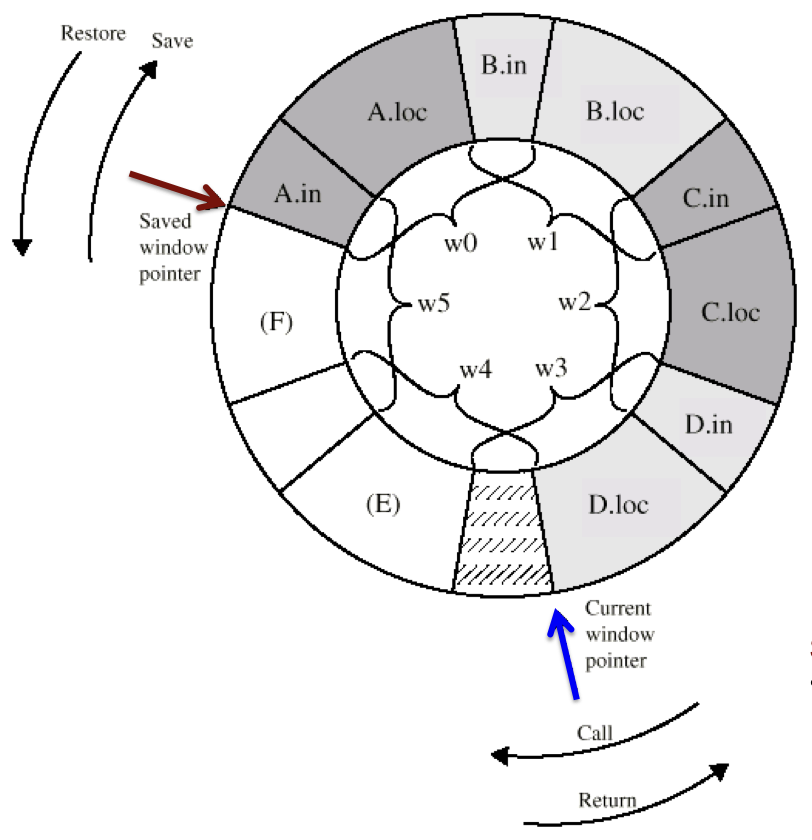
\includegraphics[scale=0.3]{immagini/procedureannidate}
	\caption{Immagine esemplifictiva sull'uso dei registri in modo annidato.}
	\label{procedureannidate}
\end{figure}
%4

Analizzando i dati di ricerca, le aziende produttrici di computer hanno notato che una grande quantità di tempo era perso a causa di salti e brench, per questo motivo si sono concentrati nell'ottimizzazione di un'unità di controllo efficiente.\\
L'architettura CISC permette molti metodi di indirizzamento diversi, ma studiando da un punto di vista analitico l'utilizzo dei metodi effettivamente adoperati da un compilatore, si nota che è sufficiente un solo metodo di indirizzamento. In questo modo, l'hardware è semplificato e la pipeline me giova: dal momento che l'indirizzamento degli operandi è il medesimo (per tutte le istruzioni) non ci sono grandi differenze nelle tempistiche del recupero di dati tra operazioni diverse. In aggiunta, l'ottimizzazione nel recupero dei dati diventa più semplice. Queste implementazioni hanno aiutato a ridurre il prezzo della produzione di calcolatori e hanno aumentato le prestazioni. D'altro canto i programmatori si sono spostati su linguaggi ad alto livello, grazie ai quali, queste implementazioni non influenzano il loro lavoro (solamente gli sviluppatori di linguaggi ed in particolare di compilatori devono cambiare il proprio approccio.\\
%
%Negli anni `70 è stata introdotta l'architettura RISC (Reduced Instruction Set Computer). (Turing Award).
%L'hardware è costoso, ma il progresso tecnologico aggira questo problema. D'altro canto, anche l'evoluzione del software è molto importante ed è molto più costosa. Infatti per produrre software bisogna pagare moltissimi sviluppatori. Per questo motivo si sono svilluppati linguaggi di alto livello che possono essere trascritti facilmente. I linguaggi di alto livello hanno il pro che sono molto semplici da imparare. Il compilatore traduce il linguaggio ad alto livello in codice assembler. \\
%Paradigmi di programmazione:
%\begin{enumerate}
%	\item imperativo;
%	\item object-oriented;
%	\item logico;
%	\item funzionale;
%\end{enumerate}

%Per non pesare sul compilatore è stata introdotta la tecnologia CISC, per cui non c'erano problemi di traduzione: tutte le operazoni che erano possibili come method() sono state implementate sull'hardware. Sono possibili tutti i metodi di indirizzamento e tutti i formati di istruzione. Pro: semplificare il lavoro del compilatore. Migliore efficienza di esecuzione. \\Contro: alta complessità di realizzazione e di implementazione. Il compilatore aveva una possibilità di scelta molto ampia: rallentava il lavoro del compilatore. \\

%Inizio anni `70, individuare le caraterristiche e i pattern dell'hardware ad alto livello, per vedere le operazioni che erano più eseguite. Tipo e frequenza d'uso degli operandi: qual'è il miglior metodo di organizzamento della memoria. Flusso di esecuzione.\\Questo studio è stato eseguito analizzando il codice assembler di un programma: statico. Dinamico: si analizza lo svolgimento del programma.

%\begin{itemize}
%	\item trasferimento dei dati;
%	\item controllo dei loop e dei salti;
%	\item quali istruzioni rischiedono più tempo per essere svolte.
%\end{itemize}

%Per esempio, una grande parte del tempo dell'esecuzione di un programma scritto in Pascal, si riferisce all'assegnamento di un valore ad una variabile; invece in C è il comando if. Studiando vari programmi si notava che gli annidamenti non sono così presenti.

%Per qusto motivo è stato pensata un'architettura che non rende il linguaggio macchina più simile al linguaggio ad alto livello. Inoltre si notava che è di gran lunga meglio ottimizzare il tempo dei pattern più utilizzati piuttosto che aumentare la quantità di istruzioni.\\

%Per questo motivo sono stati implementati un grande numero di registri per ottimizzare l'accesso agli operandi: ridurre gli accessi in memoria (molto lento).\\ La pipeline è stata studiata accuratamente: gestione oculata del controllo delle istruzioni: in particolare per quanto riguarda i salti.\\ Set di istruzioni molto conciso: implementato in maniera efficiente, hardware più veloce. Microprogrammazione: prevede l'accesso in memoria per tradurre il codice oprativo, prende una grande quantità di tempo. Ironicamente il circuito è parecchio più corto, per questo motivo il segnale viaggia attraverso un percorso più breve e quindi giunge più rapidamente.\\

%Implementazione della nuova architettura:
%\begin{enumerate}
%	\item più registri, implementazione software: il compilatore deve ottimizzare l'uso dei registri:\\	Ad ogni operazione è assegnato un gruppo di registri: una finestra. Se un'operazione a deve leggere dei registri di un'operazione b, allora la finestra di b diventa la finestra di a, l'operazione a lavora e salva i dati nella finestra di b e poi l'operazione b continua ad eseguire istruzioni in quella finestra, se è richiamata;
%	\item cosa succede se si verifica un livello di annidamento molto grande: c'è un numero massimo di istruzioni annidate possibili. Se si finiscono i registri, i registri iniziali sono salvalti in memoria (si riprende l'idea del loop buffer, buffer circolare), la figura \ref{procedureannidate} è esemplificativa del processo adoperato per liberare i registri. Si può svolgere fino a 6 operazioni annidate perchè con il pattern studiato si vedeva che 6 operazioni annidate è il livello di annidamento che permette di risolvere gran parte dei casi. Notare che il programmatore non può indirizzare direttamente i registri.
%\end{enumerate}


Il numero maggiore di registri permette di effettuare più operazioni aritmetico-logiche di seguito senza alcun bisogno di salvare i dati in memoria. Per interagire con lo storage è necessario aggiungere un'apposita istruzione; questo riduce molto il numero di istruzioni, aumenta la frequenza di esecuzione delle istruzioni e accorcia le istruzioni: ci sono meno istruzioni e quindi sono necessari meno bit per indicare un'operazione, il metodo di indirizzamento è solo del tipo registro diretto, per cui sono sufficienti pochi bit; tra l'altro è possibile utilizzare anche altri metodi di indirizzamento combinando più istruzioni. Per cui anche il formato delle istruzioni diventa più semplice (meglio per la pipeline).\\
In un programma sono richieste variabili globali, che non cambiano nel corso del programma.
Le variabili globali sono salavate in registri ad hoc in modo tale che siano accessibili da tutte le funzioni. \\
Nei linguaggi ad alto livello, il programmatore non inizializza un dato in un registro, il compilatore si occupa di ottimizzare l'utilizzo dei registri. Il numero dei registri è finito, per questo motivo è necessario ottimizzare l'utilizzo dei registri; questo vale in modo particolare per le architetture RISC che fanno un largo uso di queste memorie.
In particolare tutte le informazioni sono salvate in registri simbolici, infiniti, ma non reali. Il compilatore deve analizzare l'utilizzo dei dati per salvare più informazioni possibili nei registri; nel momento in cui sono necessarie più informazioni del numero di registri allora l'operando è salvato in memoria. Salvare i dati in memoria rallenta molto un computer.

\begin{table}[h]
	\centering
	\begin{tabular}{|l l l|}
		\hline
			& & \\
		  & \textbf{Complex Istruction Set Computer} & \textbf{Reduced Instruction Set Register} \\
			& & \\
		1 & hardware complesso & hardware semplice \\
	 	2 & molte operazioni   & poche operazioni  \\
		3 & pochi registri     & tanti registri    \\
		4 & lunghezza delle istruzioni variabile & lunghezza delle istruzioni fissa \\
		5 & istruzioni complesse & istruzioni essenziali \\
		6 & poche istruzioni in un programma & molte istruzioni in un programma\\
		7 & programmi corti & programmi lunghi\\
		  & & \\
		\hline
	\end{tabular}
	\caption{confronto tra CISC e RISC.}
\end{table}

In linea di massima è difficile confrontare queste due architetture: le due tecnlogie sono state implementate in hardware molto diversi, inoltre, a favore della retrocompatibilità, i computer che implementavano al tecnologia CISC oggi utilizzano un processore misto; per questo motivo non è possibile affermare con certezza quale delle due teclogie sia migliore.

%Dal momento in cui i registri reali sono occupati, si utilizzano i registri simbolici. Euristiche: scartare soluzioni evidentemente scarsi. Oggi raggiungiamo ottimizzazioni sufficientemente performanti.

%%


%Comparazione RISC e CISC

%cisc: set di istruzioni molto ampio, singole itruzioni complesse. Scopo: avvicinare il livello di complessità dell'hardware al livello di complessità delle istruzioni. Non funziona sempre, è bene mettere le istruzioni di cui abbiamo bisogno nel contesto.
%Avendo un gruppo di istruzioni che sono eseguite con la pipeline: sono gestite istruzioni molto grandi e complesse nel stesso momento di istruzioni piccole e veloci: si vengono a formare delle bolle. Molti programmi in CISC specificano indirizzi nella memoria principale. Mentre la peculiarità dell'architetture RISC riguarda l'utilizzo dei registri.

\section{I Processori MIPS}

Adduciamo l'esempio dei processori della famiglia MIPS per analizzare il funzionamento di un elaboratore con architettura RISC.\\
I processori MIPS utilizzano istruzioni lunghe 32 bit. Tutte le operazioni svolte dal processore sono svolte attraverso i registri, questo sistema non è molto flessibile, ma permette di velocizzare la pipeline: riduce le "bolle". Le operazioni LOAD e STORE sono svolte da una partizione della CPU a sé stante, che permette una comunicazione veloce con la memoria;
% Con l'avvento di questa tecnlogia la pipeline si è evoluta: \textit{superscalar architecture}, sono introdotti dei registri in grado di salvare due o tre output di un esecutore, in modo tale da eseguire istruzioni piccole in contemporanea con istruzioni grandi perdendo una minore quantità di tempo; \textit{superpipelined architecture}: la pipeline è divisa in fasi molto piccole, in modo tale da svolgere molte più operazioni nel medesimo arco di tempo.
In questa architettura ci sono 32 registri ad uso generale, ciascuno a 32 bit; il registro \$0 contiene la costante 0, ovvero tutti e 32 i bit di questo registro hanno valore 0.\\
Ricapitolando i metodi di indirizzamento sono:
\begin{enumerate}
	\item Registro: per tutte le operazioni;

	\item Immediato: per tutte le operazioni;

	\item Spiazzamento: per le operazioni di salto o di store o load.
\end{enumerate}

Inoltre sono presenti tutte le modalità da esse derivabili: indiretta registro (spiazzamento con il dato immediato = 0) e diretto (la base è contenuta nel registro \$0).

\subsection{Il formato delle Istruzioni}

Questa architettura supporta tre formati per rappresentare le istruzioni; tutti hanno in comune una cosa: il campo opcode è lungo 6 bit, questo permette di ottimizzare la pipeline: è possibile decodificare immediatamente il codice operazionale. I tre formati sono:

\begin{enumerate}
	\item \textbf{Formato R}: 5 bit RS, registro sorgente; 5 bit RT, registro target, 5 bit RD, registro destinazione; 5 bit per un eventuale shift dei registri (non so cosa voglia dire); 6 bit funzionale, per la variabile funzionale. In particolare RS e RT sono i registri in cui sono contenuti gli operandi dell'operazione; mentre nel registro RD è salvato il risultato, questi registri possono coincidere. I 6 bit finali servono per specificare l'operazione: per esempio se è effettuta una somma si specifica se la somma è tra integer oppure tra float;

	\item \textbf{Formato I}: 5 bit RS, registro sorgente; 5 bit RT, registro target; 16 bit Imm, dato immediato. In questo caso è effettuata un'operazione tra l'RT e Imm ed il risultato è salvato in RT, se si tratta di un'operazione logico aritmetica; altrimenti in caso di LOAD nel registro target è salvato il dato recuperato dalla memoria, mentre l'operazione tra RS e Imm permette di ottenere l'indirizzo in cui è salvato il dato che vogliamo recuperare. Ci sono altri casi, ma lo vedremo meglio più avanti;

	\item \textbf{Formato J}: 16 bit Imm, per il campo immediato. Questo formato è pensato ad hoc per il salto incondizionato: il campo Imm è moltiplicato per 4 (l'indirizzamnto è al byte), in questo modo si saltano il numero di istruzioni scritto nel campo Imm.
\end{enumerate}

\subsection{La Pipeline}
Questa architettura è ottimizzata per avere una pipeline molto efficiente, infatti MIPS vuole dire \textit{microprocessor without interclock pipeline stages}. In realtà la pipeline dell'archittettura MIPS è dotata di 5 fasi: IF, \textit{instruction fetch}, ID, \textit{Instruction Decode}, EX, \textit{Execute}, MEM, \textit{Memory Access}, WB, \textit{write-back}. Le fasi sono ottimizzate in modo tale da diminuire i tempi morti al minimo.
Analiziamo che cosa accade in ogni fase:
\begin{enumerate}
	\item IF, \textit{Instruction Fetch}: come si intuisce dal nome di questa fase, è effettuato il fetch dell'istruzione, per cui il contenuto del PC è copiato nel MAR ed è trasmesso alla memoria, che restituisce l'istruzione. L'istruzione è salvata nell'IR. In contemporanea è aggiornato l'NPC: $NPC = PC + 4$. L'NPC è un registro temporaneo, è introdotto per migliorare le prestazioni nel caso in cui ci sia un'operazione di salto condizionato. Viene incrementato di 4 perchè si saltano 4 byte: si passa all'istruzione successiva;

	\item ID, \textit{Instruction Decode}: si analizza l'operazione. Nel caso in cui il formato sia R: si accede ai registri indicati da RS e RT e i loro contenuti sono trasferiti nei registri A e B.\\
	Se si tratta del formato I: si accede ai registri indicati dai campi RS e RT e il loro contenuto è spostato in A e B, mentre il contenuto del campo immediato è trasferito nel registro temporaneo Imm., il valore salvato nel campo immediato è adattato alla lunghezza del registro Imm.: 32 bit.\\
	Nel qual caso il formato sia J: allora il campo immediato è trasferito nel registro Imm., dopo che è stato allungato fino a 32 bit. Inoltre è shiftato di due posizioni a sinistra: equivale all'operazione $\cdot 4$;

	\item EX, \textit{EXecute}: nel caso in cui si stia lavorando con il formato R, è eseguita l'operazione tra i valori nei registri A e B ed il risultato è salvato nel registro temporaneo ALUoutput; \\
	Se si si esegue un'istruzione nel formato I, allora si esegue l'operazione tra i contenuti dei registri A (ex RS) e Imm., ancora una volta il risultato è salvato nel registro ALUoutput.\\
	Se si tratta di un'istruzione di salto incondizionato e quindi il formato dell'istruzione è il J, allora è eseguita la somma tra il contenuto del registro Imm. e l'NPC (incrementato di 4). Il conteuto in questo caso è salvato nel registro target, in modo tale che il salto avvenga velocemente.\\
	In particolare nel qual caso si esegua un'istruzione di salto condizionato è eseguito il confronto tra i registri A e B, se i due valori sono uguali allora il contenuto del registro Imm. è sommato all'NPC ed il risultato è salvato nel registro target.\\

	\item MEM, \textit{MEMory access}: questa fase viene saltata nel caso in cui si esegua un'istruzione logico-aritmetica. Nel caso del salto (ormai non è più importante che il salto sia condizionato o meno) il contenuto del PC è sovrascritto con l'indirizzo memorizzato dall'RT.\\
	Nel caso del LOAD, l'indirizzo ottenuto nella fase EX è mandato nel MAR e poi alla memoria, che rimanda il contenuto della cella di memoria indicata all'LMD, il \textit{Load Memory Data Register}.\\
	Nel caso della STORE il dato nel registro A (ex RS) è mandato all'indirizzo in memoria calcolato nella fase precedente;

	\item WB, \textit{Write-Back}: se si effettua la LOAD, il contenuto del registro temporaneo LMD è trasferito nell'RT. \\
	Altrimenti, nei casi di operazioni registro-registro oppure registro-dato immediato, il valore memorizzato nell'ALUoutput è trasferito nei rispettivi registri RD oppure RT.
\end{enumerate}

\subsection{I Registri delle Fasi della Pipeline}
Quando ho descritto la pipeline, abbiamo visto che per un corretto funzionamento della pipeline è necessario introdurre dei registri tra le varie fasi della pipeline. In questa subsection analizziamo i registri che si trovano tra le fasi della pipeline che caratterizzano l'architettura MIPS:
\begin{enumerate}
	\item \textbf{IF/ID}:
		\begin{itemize}
			\item IF/ID.IR $\leftarrow$ Memoria[PC]: si trasferisce l'istruzione nella cella di memoria individuata dal PC nel registro IR di questa fase;
			\item IF/ID.NPC $\leftarrow$ PC + 4 (prossima istruzione);
		\end{itemize}

	\item \textbf{ID/EX}:
		\begin{itemize}
			\item ID/EX.IR $\leftarrow$ IF/ID.IR: si trasferisce l'istruzione dal registro IR della fase precedente a quello della fase attuale, ogni fase è dotata del registro IR;

			\item ID/EX.A,B $\leftarrow$ IF/ID.IR[RS, RT];

			\item ID/EX.Imm $\leftarrow$ IF/ID.IR[campo immediato]: il campo immediato è trasferito in questo registro; in caso di salto il valore in esso contenuto è shiftato di due posizioni a sinistra ($\cdot 4$), in modo tale che il valore indicato rappresenti il numero di istruzioni da saltare; idem per quanto riguarda gli indirizzi. Resta uguale solo nel caso si esgua un'operazione aritmetico-logica;

			\item ID/EX.NPC $\leftarrow$ IF/ID.NPC;
		\end{itemize}

	\item \textbf{EX/MEM}:
		\begin{itemize}
			\item EX/MEM.IR $\leftarrow$ ID/EX.IR;

			\item Operazioni logico-aritmetiche:
				\begin{itemize}
					\item EX/MEM.ALUoutput $\leftarrow$ (ID/EX.A operazione ID/EX.B oppure ID/EX.Imm);
				\end{itemize}

			\item LOAD e STORE:
				\begin{itemize}
					\item EX/MEM.ALUoutput $\leftarrow$ (ID/EX.A + ID/EX.Imm);

					\item EX/MEM.B $\leftarrow$ ID/EX.B;
				\end{itemize}

			\item salto:
				\begin{itemize}
					\item EX/MEM.Target $\leftarrow$ (ID/EX.NPC + ID/EX.Imm);

					\item EX/MEM.Cond $\leftarrow$ (ID/EX.A - ID/EX.B): se viene 0 allora viene effettuato il salto;
				\end{itemize}
		\end{itemize}

	\item \textbf{MEM/WB}:
		\begin{itemize}
			\item MEM/WB.IR $\leftarrow$ EX/MEM.IR

			\item In questa fase le operazioni logico-aritmetiche non hanno di svolgere alcuna funzione:
			\begin{itemize}
				\item MEM/WB.ALUoutput $\leftarrow$ EX/MEM.ALUoutput;
			\end{itemize}

			\item LOAD:
				\begin{itemize}
					\item MEM/WB.LMD (\textit{laod memory data register}) $\leftarrow$ Memoria[EX/MEM.ALUoutput];
				\end{itemize}

			\item STORE:
				\begin{itemize}
					\item Memoria[EX/MEM.ALUoutput] $\leftarrow$ EX/MEM.B (target);
				\end{itemize}

			\item salti: alla fine di questa fase i registri sono vuoti, ma alcuni dati sono trasferiti durante questa fase:
			  \begin{itemize}
			 	 \item EX/MEM.IR: verifica che l'istruzione attuale sia di salto;

				 \item EX/MEM.Target $\rightarrow$ PC, se la condizione successiva è verificata;

				 \item EX/MEM.Cond: il valore è portato alla fase IF; se è 0, grazie ad un transistor il registro target sovrascrive il PC;
			  \end{itemize}
		\end{itemize}

	\item \textbf{WB}:
		\begin{itemize}
			\item Operazioni logico-aritmetiche:
				\begin{itemize}
					\item Registro[MEM/WB.IR[RD/RT]] $\leftarrow$ MEM/WB.ALUoutput;
				\end{itemize}

			\item LOAD:
				\begin{itemize}
					\item Registro[MEM/WB.IR[RT]] $\leftarrow$ MEM/WB.LMD: è salvato il dato caricato dalla memoria nel registro indicato nel campo RT (\textit{register target});
				\end{itemize}
		\end{itemize}

		\item Sia STORE che i salti sono già completate.
\end{enumerate}

\begin{figure}[h]
	\centering
	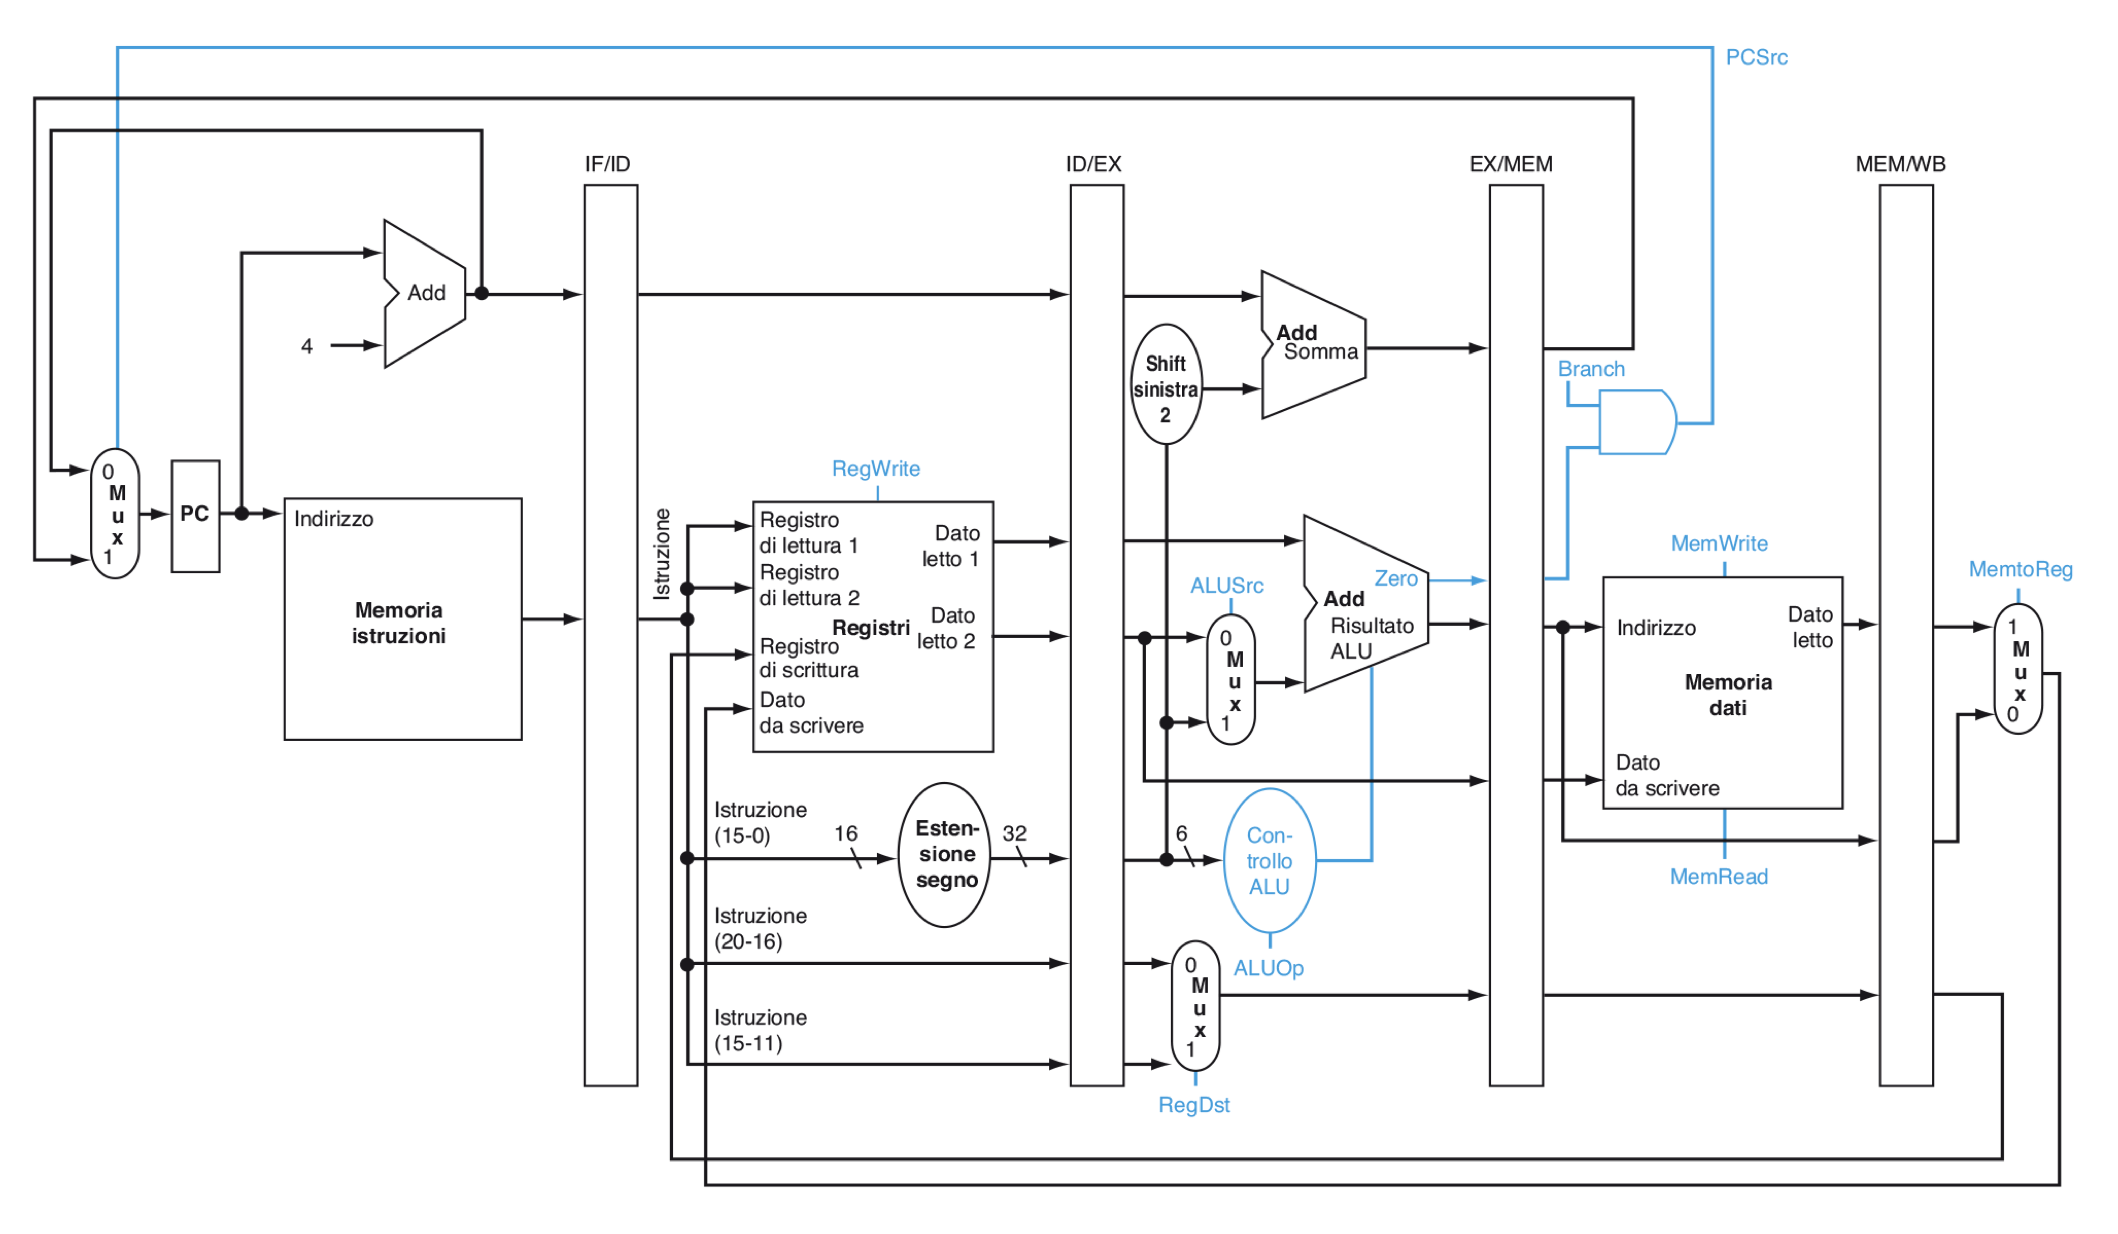
\includegraphics[scale=0.2]{immagini/hardwaremips}
	\caption{rappresentazione schematica di un processore ad architettura MIPS.}
	\label{hardwaremips}
\end{figure}

La \autoref{hardwaremips} è una buona rappresentazione delle varie componenti hardware di un processore mips, più che altro dal punto di vista della pipeline: mancano i registri nella CPU e l'unità di controllo.

\subsection{La Gestione delle Dipendenze nell'Archittettura MIPS}
Nell'architettura MIPS, è completata un'istruzione ad ogni ciclo di clock. Notare che alcune fasi non sono necessarie ad alcune le istruzioni, per questo motivo una parte del tempo viene perso, tuttavia la pipeline è molto ottimizzata. Infatti non solo le varie fasi hanno una durata simile, in più ogni ciclo di clock è diviso in due: nella prima metà è eseguito il write, mentre nella seconda metà sono letti i dati dai vari registri, read; questo accorgimento permette di risolvere moltissime problematiche legate alla dipendenza dei dati.\\
In questa architettura il WAR e il RAR non sono un problema, come qui sopra evidenziato, il ciclo di clock è diviso in due parti, la prima è la scrittura, la seconda è la lettura, per questo motivo un dato è letto nella fase precedente a quella in cui è ricritto e dunque le risorse non si sovrappongono; per quanto riguarda il Read After Read, istruzioni diverse non hanno bisongo di leggere il medesimo registro nello stesso momento: il fetch degli operandi è eseguito sempre e solo nell'ID. D'altro canto nel caso di operazioni dipendenti da istruzioni precedenti, il RAW, può rivelarsi problematico. Evidenziamo il caso in cui LOAD è posta di seguito ad un'operazione che ha bisogno dei dati prelevati dalla LOAD: in questo caso i dati sono disponibili solo dopo metà della fase MEM, quando si sono prelevate le informazioni. D'altro canto, il ciclo di esecuzione di un'istruzione richiede quei dati durante la fase ID. Questo vuol dire che è necessario mettere in pausa tutti i cicli di istruzione successivi a quello di LOAD, perchè il dato necessario arrivi in tempo. Si dice che è effettuto un \textbf{data forward} del dato: l'informazione necessaria è condivisa ad un altro ciclo di esecuzione (di un'istruzione) prima che l'istruzione col dato sia conclusa. In questo modo, la pipeline è sospesa solamente per un ciclo di clock.\\
Nel caso in cui un'operazione modifichi un dato che è richiesto dall'istruzione successiva, invece è suffuciente effetture un \textit{data forward} in concomitanza con la fase \textit{execute} della prima istruzione verso l'\textit{instruction decode} della successiva: le due fasi sono successive ed il dato, invece che essere salvato nell'EX/MEM.ALUoutput è mandato al registro richiesto: ID/EX.A oppure ID/EX.B. Notare che in questo caso non si generano bolle.\\
Nel caso in cui ci sia la STORE di un registro non si genera alcun problema, poiché il dato non è modificato.\\
Se si effettua un salto, il fetch dell'istruzioni avviene nella fase \textit{istruction fetch} mentre è eseguita la fase MEM dell'istruzione di salto.

%rs: registro sorgente (primo operando)
%rt: registro target (secondo operando)
%rd: registro destinazione (dove salvare il risultato)
%shamt:
%funct:

%
%
%rs: registro base
%address/ const: Spiazzamento
%rt: dove salvare il dato

%spiegare write through e write back e write allocate!

\end{document}
